\chapter{Evaluation}\label{chap:evaluation}

\section*{}

\minitoc \mtcskip \noindent
This section evaluates how the solution developed provides evidence towards the validity of hour hypothesis presented in \sectionref{sec:main_hypothesis} and fulfills the requirements presented in \sectionref{sec:desiderata}. \sectionref{sec:scenarios} proposes scenarios \sectionref{sec:experiments} proposes the experiments that will be used to evaluate the developed solution. \sectionref{sec:evaluation_discussion} discusses the results of the experiments and rreaches conclusions regarding their success. \sectionref{sec:evaluation_hypothesis} evaluates the veracity of the main with the evaluation data. Finally, \sectionref{sec:evaluation_lessons_learned} reflects on the lessons learned during the evaluation process. 

\section{Scenarios}\label{sec:scenarios}

To validate to which extent we were able to reach the goals as mentioned earlier \seesectionref{sec:motivation}, we proceed to evaluate our architecture and \textit{proof-of-concept} in both virtual --- using Docker with a Unix-compatible version of MicroPython --- and physical setups --- using both ESP8266 and ESP32 connected in the same Wi-Fi network.

The experiments were performed in a computer with an i5-6600K at 3.5GHz processor, with 16Gb of RAM and running Linux Manjaro kernel version 5.6.16. The base Node-RED was version 1.0.6, Mosquitto MQTT broker at version 1.6.10 and MicroPython firmware at version 1.12.

We outline the following two experimental scenarios as a foundation for our experiments:

\begin{description}
    \item[\textbf{ES1}] A room has three sensors that give temperature and humidity readings every minute. There is a virtual sensor that compares the results (of both temperature and humidity) and triggers depending on configured thresholds. An AC unit must be provided with the comparison result to define both (a) if it \textit{switches on/off}, and (b) its operating mode: \textit{cool}, \textit{heat}, and \textit{dehumidify}, all mutually exclusive. The Minimal Working System (MWS) consists in (a) one temperature sensor, (b) one humidity sensor, (c) one \textit{node} capable of making the decision, and (d) working communication channels amongst them.
    \item[\textbf{ES2}] A system contains 20 devices that are responsible for propagating an injected message amongst themselves to their final output. In the end, the injected message must reach the specified MQTT topic.
\end{description}

\begin{figure}[h]
\centering
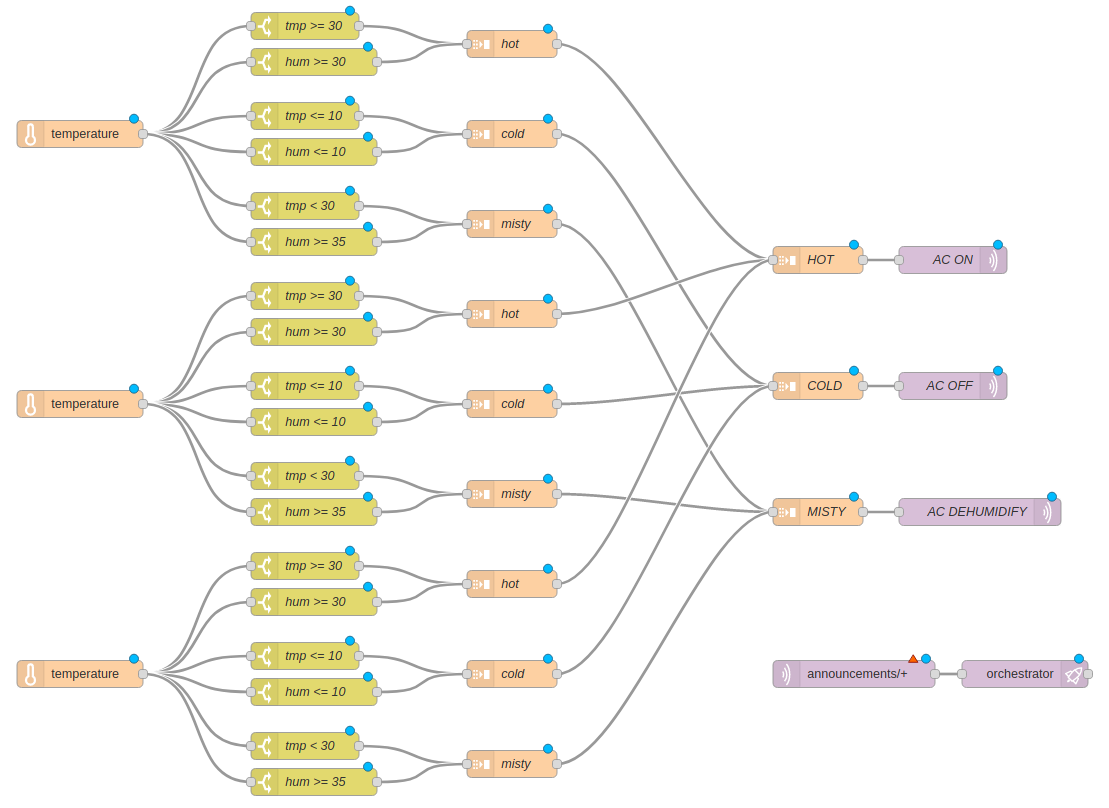
\includegraphics[width=\textwidth]{scenario1.png}
\caption[Node-RED implementation of scenario 1]{Node-RED implementation of scenario 1}\label{fig:scenario1_node_red}
\end{figure}

\textbf{ES1}, which resembles a real-world scenario, aims to test the features of the developed solution with a moderately simple Node-RED \textit{flow} \seefigureref{fig:scenario1_node_red}, taking advantage of the \textit{nodes} developed for MicroPython code generation support. As a complement, \textbf{ES2} allows the comparison of the developed solution to the already existing ones by implementing the same scenario in different environments. For each one of the experimental scenarios (\ie \textbf{ES1} and \textbf{ES2}) we defined a set of experimental tasks. 

\section{Experiments}\label{sec:experiments}

\subsection{ES1 experiments}

For \textbf{ES1} two Sanity Checks were performed, one over virtual devices --- Sanity Check 1 (\textbf{ES1-SC1}) --- and other with physical devices --- Sanity Check 2 (\textbf{ES1-SC2}). A set of readings and message forwarding tasks were performed with no compensation or any other fault-tolerance strategies. Each sensor device only provided environmental readings to the system. Orchestration is centralized. We expect all roundtrips to take less than the smallest part that can be resolved (measurement capability, which we estimate to be $<1$ second).

We further defined a set of (re-)orchestration experiments for \textbf{ES1}, where the system must allocate computation tasks among the available resources (\ie devices), namely:
\begin{description}
    \item[ES1-A] MWS is achieved via multiple possible configurations by selective (provoked) device failure (fail-stop) using only virtual devices (\ie Docker);
    \item[ES1-B] MWS is achieved via multiple possible configurations by selective (provoked) device failure (fail-stop) using physical devices;
    \item[ES1-C] Inconsistent device behaviour, \eg appear and disappear in shorter intervals lower than the time needed for orchestrating convergence (OCT), that leads to activity impacting the MWS. An orchestrating converge consists in an assignment of \textit{nodes} to devices that result in a working system; 
    \item[ES1-D] With 4 devices, each one with different processing capabilities. During orchestration, some devices will develop an out-of-memory error because they cannot process all the processing tasks assigned to them, specifically the size of the given script. The orchestrator should decide to send fewer tasks to these devices. The system is expected to converge to a working solution. \textit{This scenario will be implemented with a modified device script. When devices receive a script, it will generate a memory error if the length of the script passes a certain threshold. This crudely simulates the memory constraints of devices in various conditions.}
    \item[ES1-E] With 4 devices, some of them have a memory leak from an unknown cause. After random time \texttt{Random(t0,t1)}, these problematic devices stop working with an out-of-memory error. The orchestrator assumes that the devices cannot handle the number of processing tasks assigned to them, so in the re-orchestration, it will assign fewer tasks. Since these devices will always break, the orchestrator should eventually disconsider these devices in the assignment of nodes. \textit{This scenario will be implemented with a modified device script that will trigger an out-of-memory error after a random period, started by the execution of the given tasks.}
    \item[ES1-F] With 4 devices, there is a device that is sensitive to a particular node, which causes the device to give out an out-of-memory error. The orchestrator will potentially assign this \textit{node} to the specific device. When the device gives out the out-of-memory error, the orchestrator will eventually converge to a solution where the \textit{node} is not assigned to that particular device, and the system will converge.  \textit{These out-of-memory errors will be simulated with the use of a failure \textit{node} that forces a \texttt{MemoryException} in the device.}
    \item[ES1-G] With 50 devices, each second, the device has a probability of failing. This failure can go from 0 to 10 seconds, randomly chosen. The orchestrator must deal with the random failure of the devices and re-orchestrate the system. This experiment is considered a stress test, causing repeated failures and forcing constant re-orchestration.
\end{description}

With this set of experiments we should verify that the following constraints are meet:
\begin{enumerate}
    \item \textbf{Restrictions (predicates) are enforced.} Check that possible configurations lead to solutions that enforce defined predicates;
    \item \textbf{Priorities are honored.} Check that all specified priorities were taken into account, and only violated if necessary;
        \begin{enumerate}
            \item Priority is given to the maximum level of decentralization --- nodes spread through all the available devices --- but some centralization can occur.
        \end{enumerate}
\end{enumerate}

\subsection{ES2 experiments}

Regarding \textbf{ES2}, a total of 20 devices were connected in a line topology. A message is sent to the starting device, which will propagate it to its output. All the devices implement this propagation logic, which should result in the initial message reaching the end of the line. The propagation time is measured, starting when the message is sent and ending when the message reaches the last node. This scenario was implemented with different experimental configurations, namely:
\begin{description}
    \item[ES2-A]: Non-modified version of Node-RED, using the default \textit{node}-to-\textit{node} communication channel (\texttt{EventEmitter}), with all the \textit{nodes} sharing the same runtime;
    
    \item[ES2-B]: Modified version of Node-RED that uses MQTT as the \textit{node}-to-\textit{node} communication channel, with all the \textit{nodes} sharing the same runtime;
    
    \item[ES2-C]: MQTT-based modified Node-RED, where each \textit{node} of the \textit{flow} is assigned to a different virtual device (\ie a MicroPython-running Docker instance). The Docker instances and MQTT broker run in the same host machine;
    
    \item[ES2-D]: MQTT-based modified Node-RED, where each \textit{node} of the \textit{flow} is assigned to a different virtual device. The Docker instances share one host, but the MQTT broker is in a different one. All parts are connected to the same Wi-Fi network;
    
    \item[ES2-E]: Each physical device runs a simple script that performs the desired behaviour, on top of a non-modified MicroPython firmware image, communicating with which other over MQTT. Node-RED is not used, and there is no orchestration being performed;

    \item[ES2-F]: MQTT-based modified Node-RED, along with the modified MicroPython firmware running on physical devices. Each \textit{node} of the \textit{flow} is assigned to a different device. Each device is connected to the same Wi-Fi network and communicate between them using MQTT. 
\end{description}

%%%%%%%%%%%%%%%%%%%%%%%%%%%% DISCUSSION %%%%%%%%%%%%%%%%%%%%%%%%%%%%%%%%%%%

\section{Discussion}\label{sec:evaluation_discussion}

The scenarios and respective experimental tasks were performed, and several metrics of the system were measured. The following sections present and discuss our experimental results.

\subsection{ES1: Sanity Checks}\label{sec:discussion_scenario1}

As mentioned previously \seesectionref{sec:scenarios}, the first scenario consists of a system that controls an A/C. This system takes into account readings of 3 temperature and humidity sensors to define if the room's temperature is too hot, cold of humid and sends commands to the A/C with the respective actions.

These experiments allow us to observe that the devices can satisfy the \textit{nodes}, meaning that the system works as intended once the assignment is complete. Once this check passes, we will not verify it again in the remaining experiments.

%%%%%%%%%%%%%%%%%%%%%% SC %%%%%%%%%%%%%%%%%%%%%%

\subsubsection{ES1-SC1}\label{sec:sanity_check_exp}

This experiment was used observe the overall functionality of the approach in a controlled way (the use of virtual devices reduce the proneness to hardware-provoked failures), and the resulting assignment of \textit{nodes} can be observed in \figureref{fig:sanity_check_graph}, where the \textit{Orchestrator node} allocated nine \textit{nodes} to each device. \figureref{fig:sanity_check_node_assignment_visual} demonstrates in which devices each \textit{node} was assigned to.

\begin{figure}[h]
\centering
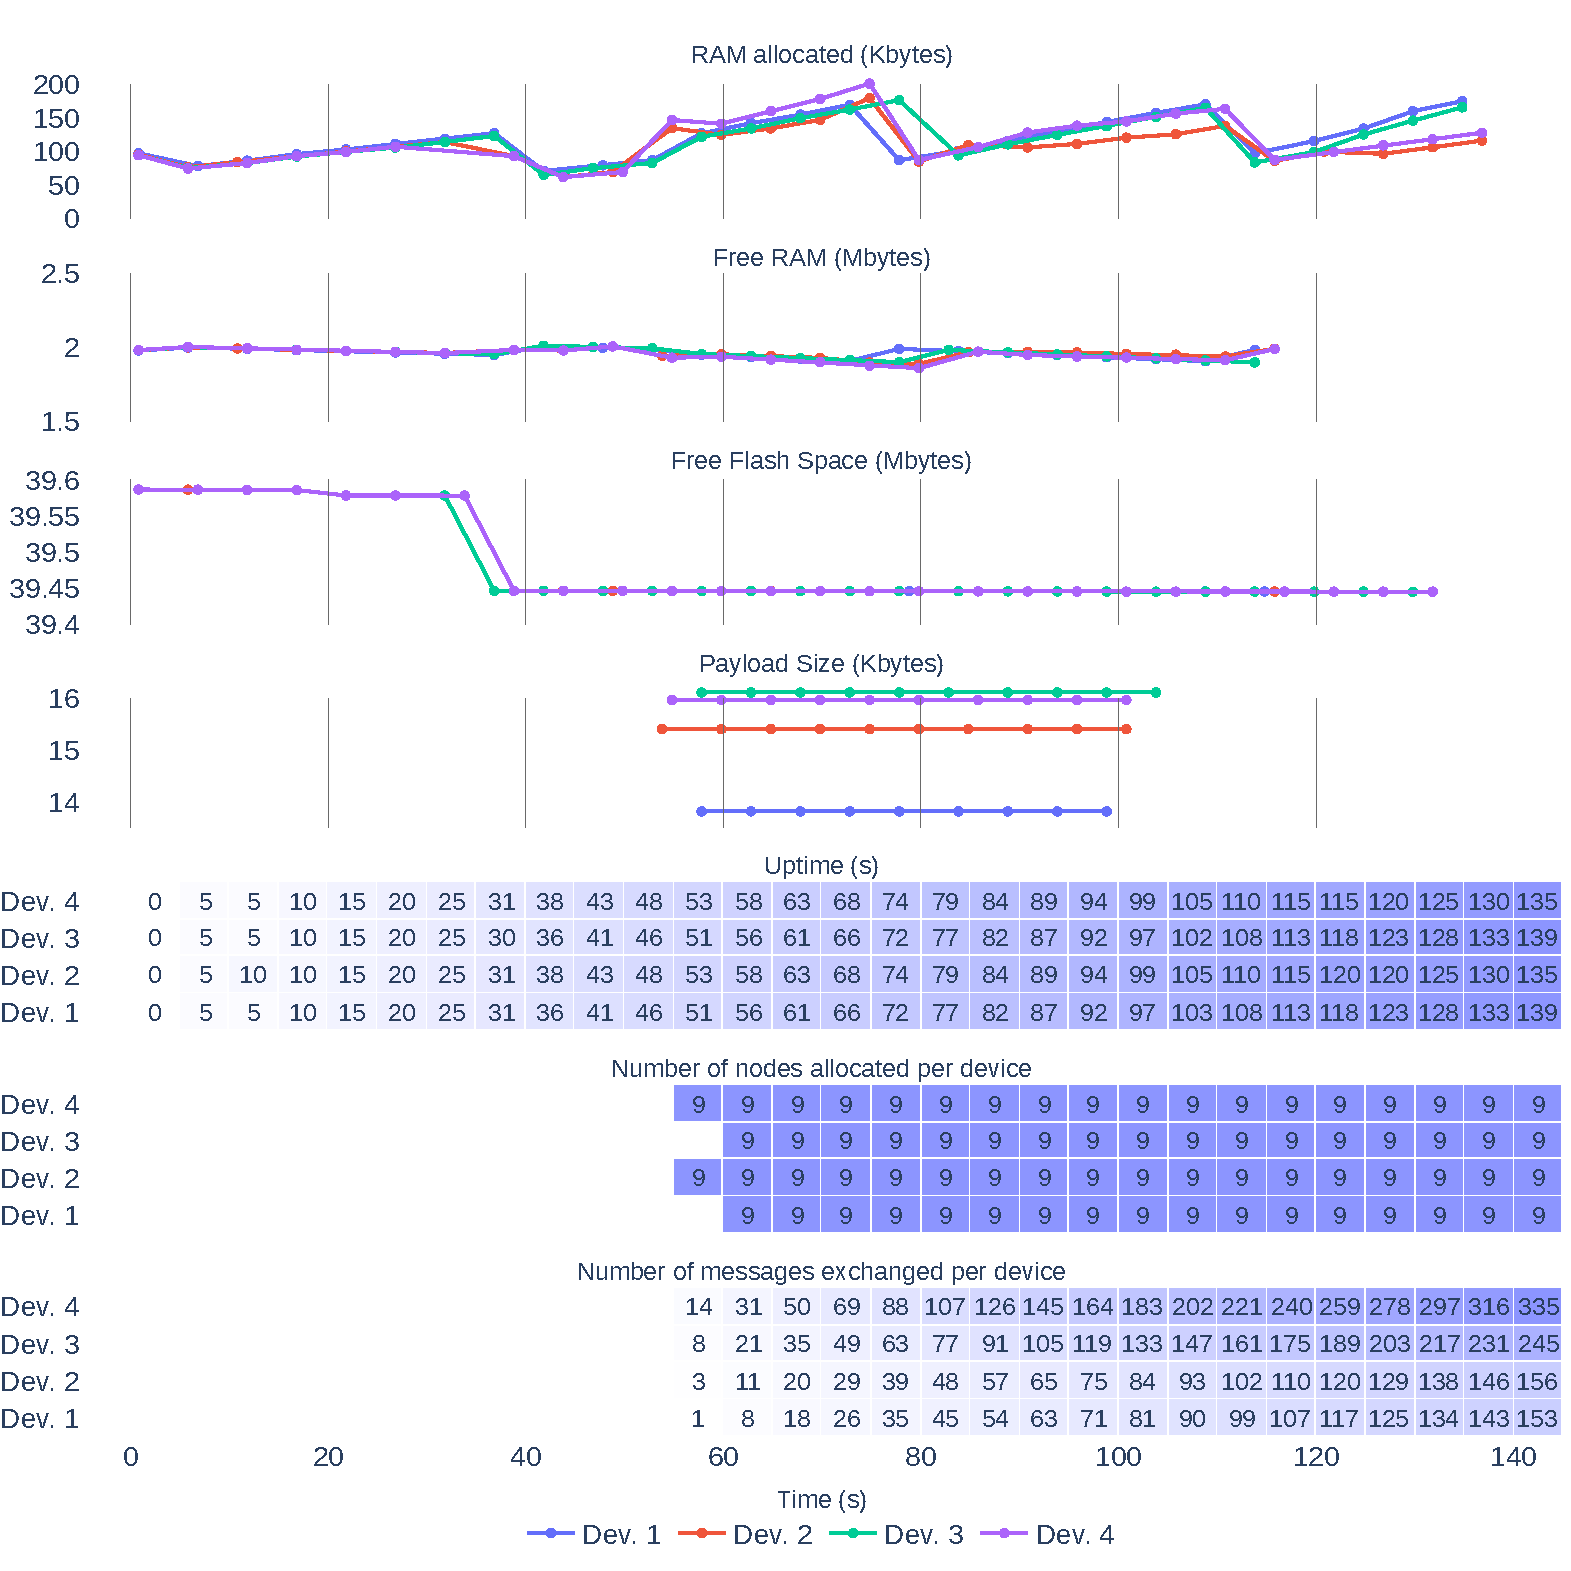
\includegraphics[width=\linewidth]{experiences/1-sanity_check/sanity_check.pdf}
\caption[ES1-SC1 measurements.]{ES1-SC1 measurements.}\label{fig:sanity_check_graph}
\end{figure}

\begin{figure}[H]
\centering
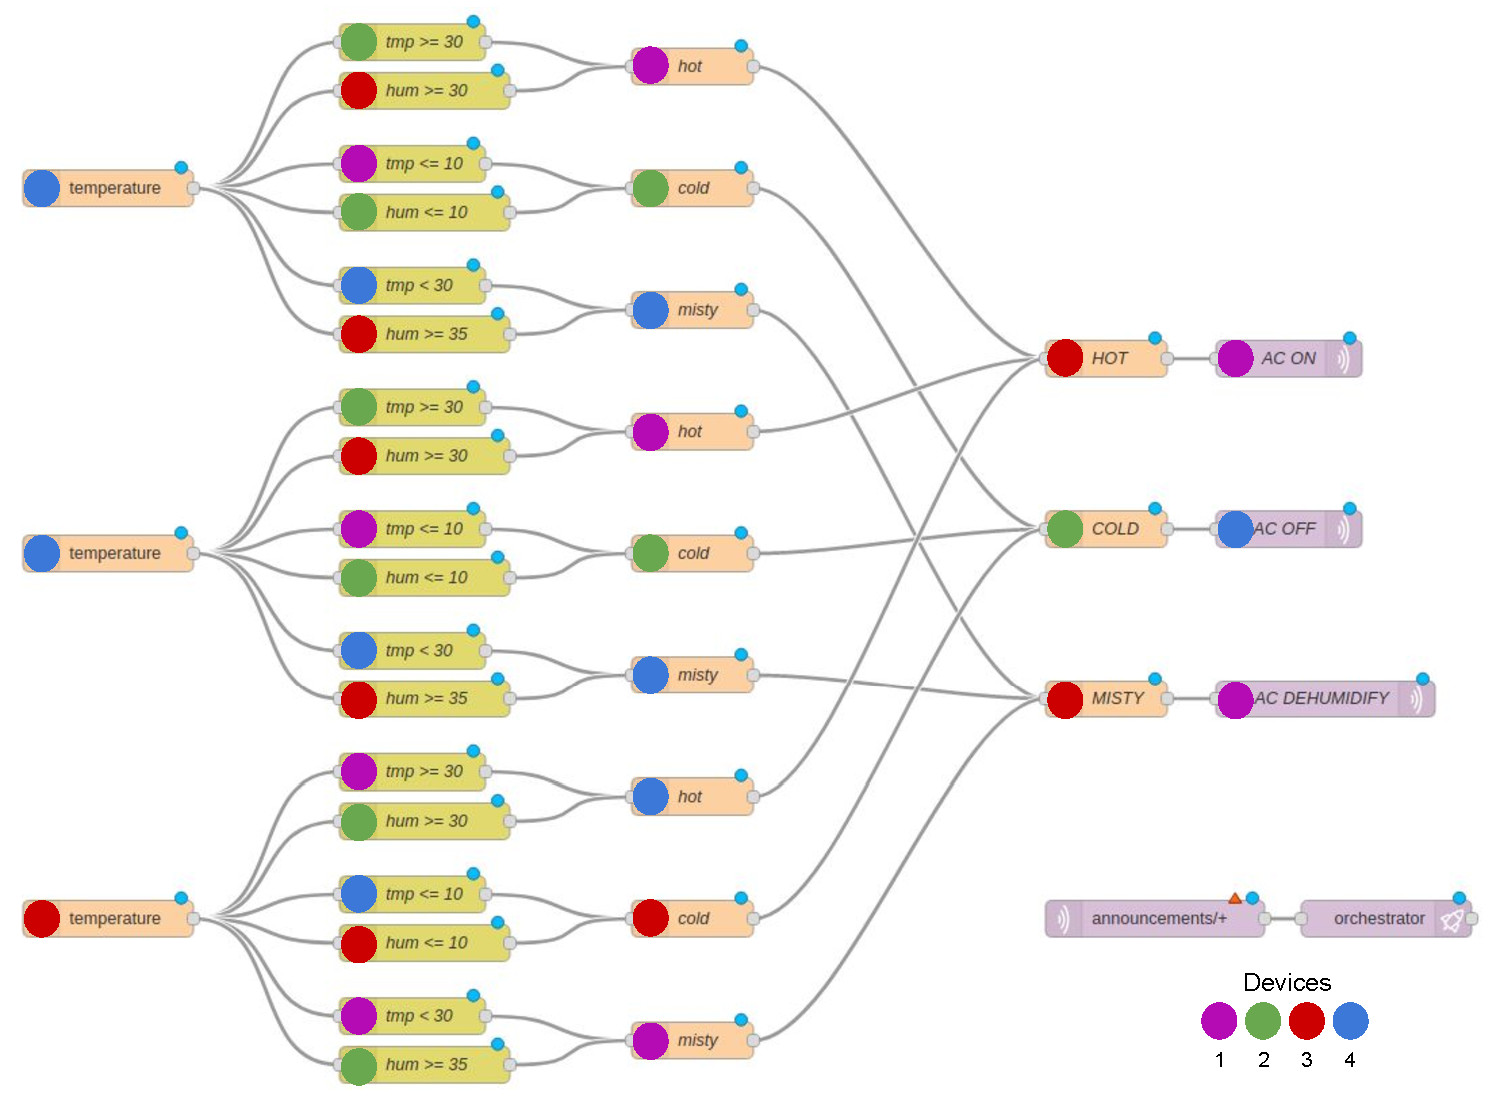
\includegraphics[width=\linewidth]{experiences/1-sanity_check/node-assignment-visual.pdf}
\caption[ES1-SC1 \textit{node} assignment.]{ES1-SC1 \textit{node} assignment.}\label{fig:sanity_check_node_assignment_visual}
\end{figure}

The usage of RAM was significant, varying from 60Kb to 200Kb \seefigureref{fig:sanity_check_graph}. The flash size only decreases to 150000 bytes when the device receives a script for executing --- matching the size of the payload received by the devices.

As the orchestrator defines the \textit{nodes} assignment, each script is built and sent to the appropriate devices. A confirmation of this delivery is necessary for the system to conclude the assignment phase and start monitoring the state of the system. The time it takes to deliver the script can be observed in \figureref{fig:sanity_check_delivery_time}. The usage of virtual devices running in the same host as the Node-RED instance allows for shorter times, which are measured in milliseconds.

\begin{figure}[H]
\centering
\includegraphics[width=\linewidth]{experiences/1-sanity_check/delivery_time_table.pdf}
\caption[ES1-SC1 script delivery time.]{ES1-SC1 script delivery time.}\label{fig:sanity_check_delivery_time}
\end{figure}

Once the devices start executing its assigned script, each allocated \textit{node} will start to communicate with each other. All the messages of all communicating topics were captured to check if the system worked as expected. This allowed us to verify that all \textit{nodes} are receiving and producing the expected output messages. The total number of communications can be consulted in \figureref{fig:sanity_check_graph}. As it can be observed, the number of messages produced by \textit{Device 4} is bigger than any other. This is due to the allocation of two temperature-humidity \textit{nodes} in this device, which publish three messages each. This number of messages published is bigger than any other \textit{node}. \textit{Device 3} contains the other temperature-humidity node \seefigureref{fig:sanity_check_node_assignment_visual}.

To verify if the script delivery time is directly related with the payload size, this experiment was repeated 10 times and the mentioned metric was measured. By analyzing \figureref{fig:delivery_times_comp}, we can observe that the delivery times between devices is very similar, with an average of $~0.303\pm0.165$s. Therefore, there is no relation between payload size and script delivery time.

\begin{figure}[h]
\centering
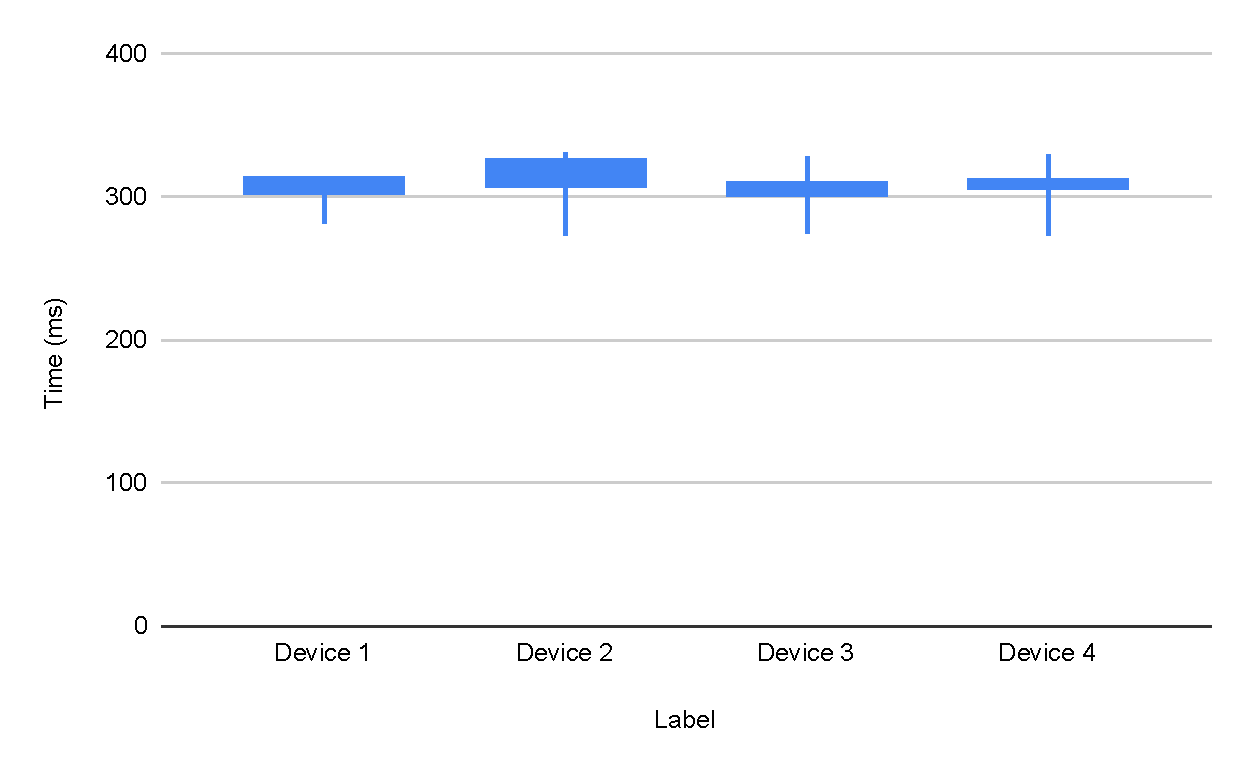
\includegraphics[width=\linewidth]{experiences/1-sanity_check/sending_script_times_comp.pdf}
\caption[ES1-SC1 delivery times.]{ES1-SC1 script delivery times.}\label{fig:delivery_times_comp}
\end{figure}

Our sanity check performs as expected in a virtual-only setup by (1) spreading the computation amongst available resources and (2) maintaining the system within expected behavior. Any errors that might occur henceforth might be due to hardware considerations.

%%%%%%%%%%%%%%%%%%%%%% SC Phys %%%%%%%%%%%%%%%%%%%%%%

\subsubsection{ES1-SC2}\label{sec:sanity_check_phys_exp}

The previous experiment was repeated using physical devices, more specifically four ESP32. Similar to the virtual devices, the assignment of \textit{nodes} to devices spread the number of \textit{nodes} equally, with each device running 9 \textit{nodes} \seefigureref{fig:sanity_check_phys_graph}.

\begin{figure}[h]
\centering
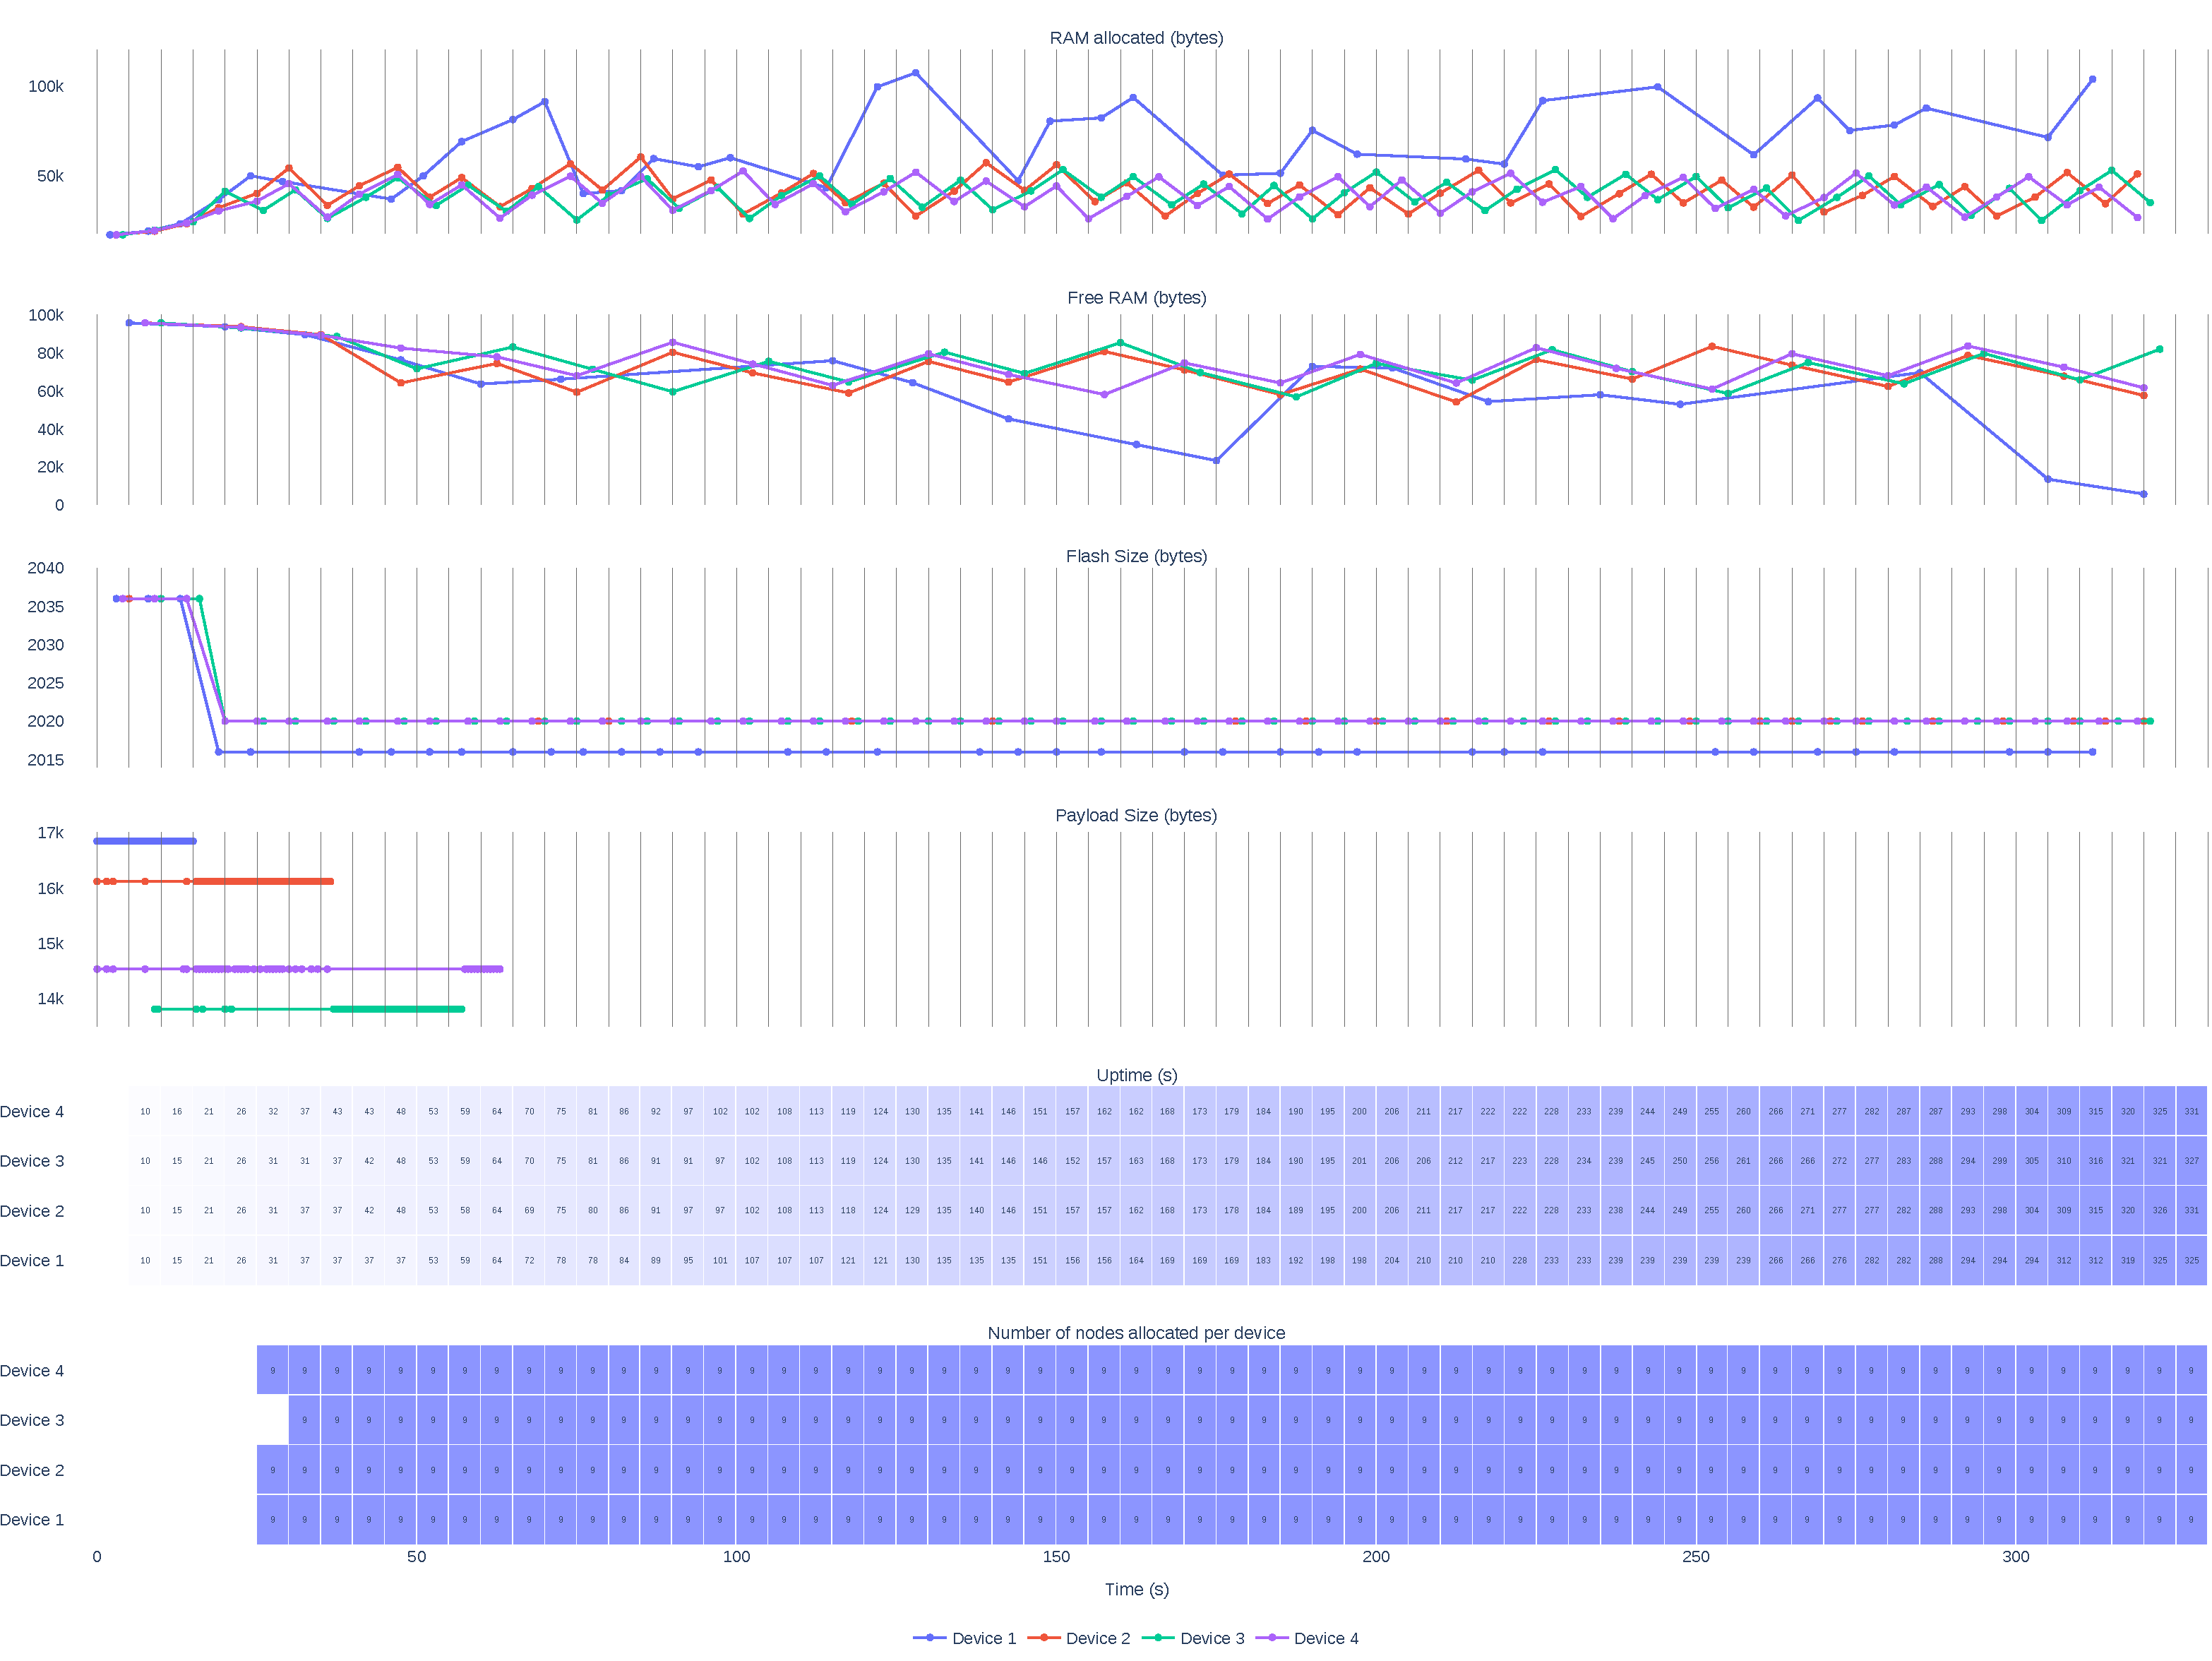
\includegraphics[width=\linewidth]{experiences/1-sanity_check_phys/sanity_check_hardware.pdf}
\caption[ES1-SC2 measurements.]{ES1-SC2 measurements.}\label{fig:sanity_check_phys_graph}
\end{figure}

The usage of RAM in physical devices is smaller than the one used by virtual devices, which can be explained with the possible optimization differences in the Docker-compatible and ESP-compatible MicroPython firmware and libraries, as well as the increased frequency of the garbage collector calls.

The free flash space of the physical devices is smaller than the virtual ones, as expected. Fig.~\ref{fig:sanity_check_phys_graph} shows that the device with the biggest payload, \textit{Device 1}, ends up having less free flash space. The overall size of the payloads is very similar to the ones in the \textbf{ES1-SC1}.

\begin{figure}[h]
\centering
\includegraphics[width=\linewidth]{experiences/1-sanity_check_phys/delivery_time_table.pdf}
\caption[ES1-SC2 script delivery time.]{ES1-SC2 script delivery timestamp.}\label{fig:sanity_check_phys_delivery_time}
\end{figure}

The script delivery time for physical devices is longer than their virtual counterpart, with an average of $~6.776\pm0.476$s \seefigureref{fig:sanity_check_phys_delivery_time}. Since the devices are not running in the same machine, the Wi-Fi stack and the devices' hardware characteristics have a non-negligible impact in the communication speed. The uptime is similar to the previous experiment since there were no hardware failures.

%%%%%%%%%%%%%%%%%%%%%% Exps %%%%%%%%%%%%%%%%%%%%%%

\subsection{ES1: Experimental Tasks}\label{sec:discussion_scenario1_exp}

These experiments focus in validating and evaluating the tool's capacity to adapt to devices' failures. Since the previous experiments \seesectionref{sec:discussion_scenario1} already verified that the devices executes the tasks that are given to them, this verification will not be repeated in this section's experiments.

%%%%%%%%%%%%%%%%%%%%%% Exp A %%%%%%%%%%%%%%%%%%%%%%

\subsubsection{ES1-A}\label{sec:exp_a}

This experiment evaluates if the system is able to re-orchestrate when a device either fails or (re-)appears (\ie new or recovered). During this experiment, devices were turned off one by one until only one was left running. It is expected that the system detects when a device has become unavailable and re-orchestrates, assigning \textit{nodes} to the available devices. In the end, only one device should be running, and all the \textit{nodes} should be assigned to it.

\begin{figure}[h]
\centering
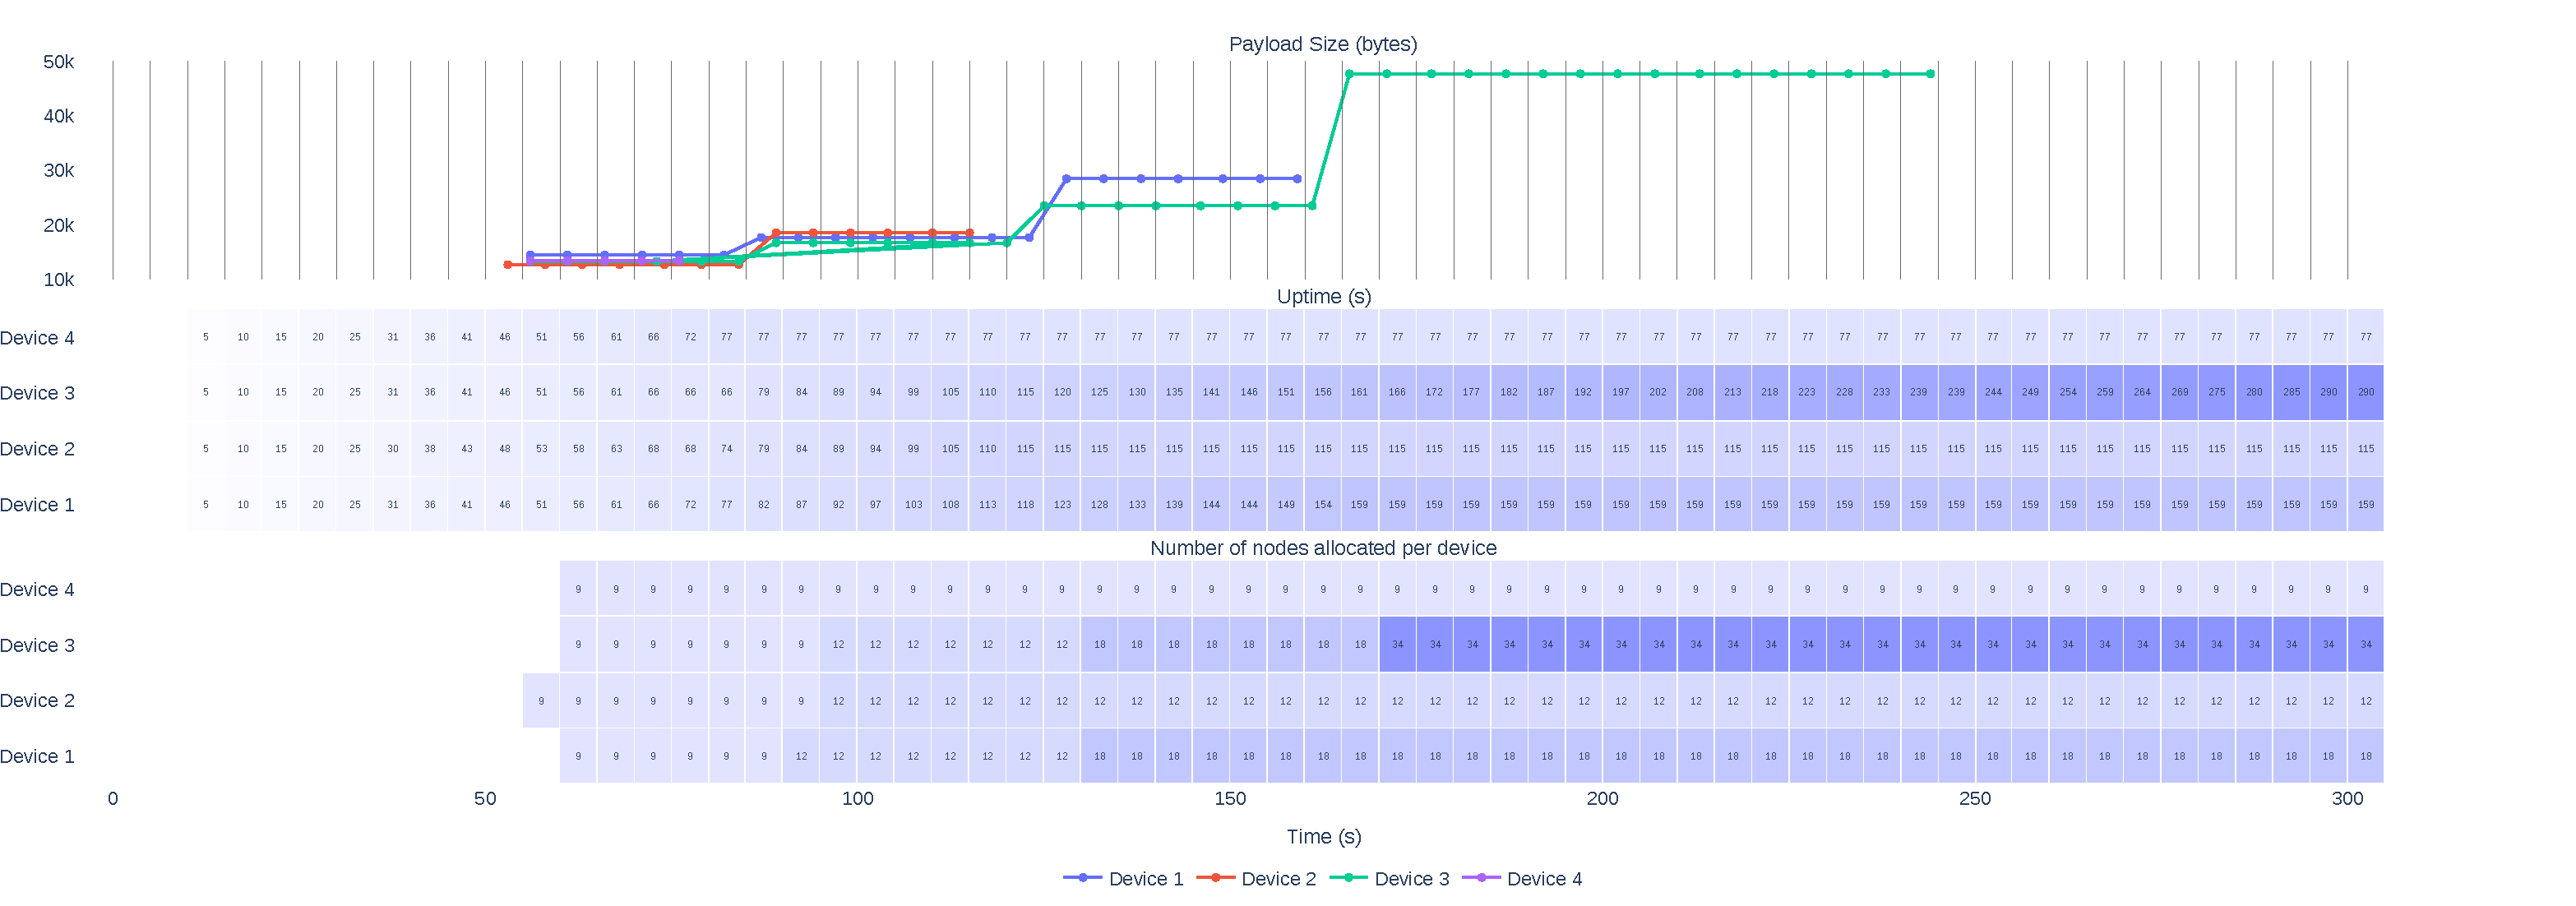
\includegraphics[width=\linewidth]{experiences/A-reorchestration/reorchestration.pdf}
\caption[ES1-A measurements]{ES1-A measurements.}\label{fig:experiment_a_graph}
\end{figure}

\figureref{fig:experiment_a_graph} shows that the uptime of the devices stops increasing one by one, identifying the moment the device fails. Once a failure happens, the system re-orchestrates, assigning the \textit{nodes} of the device to the other available devices, increasing their number \seefigureref{fig:experiment_a_graph}. The increase in the number of \textit{nodes} assigned to the available devices can also be observed in the payload size. When all devices fail except one, the one remaining receives the payload, which is higher than any other previously received.

The information regarding the number of \textit{nodes} is not updated to zero once the device fails, since it is no longer active to send the updated metric. The system identifies the failure of devices and takes actions to rectify it by repeating the assignment process, taking into account the available devices.

This allow us to verify that the system identifies the failure of devices and takes actions to rectify it by repeating the assignment process, taking into account the available devices.

%%%%%%%%%%%%%%%%%%%%%% Exp B %%%%%%%%%%%%%%%%%%%%%%

\subsubsection{ES1-B}

Based on \textbf{ES1-A} \seesectionref{sec:exp_a}, this experiment replaces the virtual devices by physical ones. 

\begin{figure}[h]
    \centering
    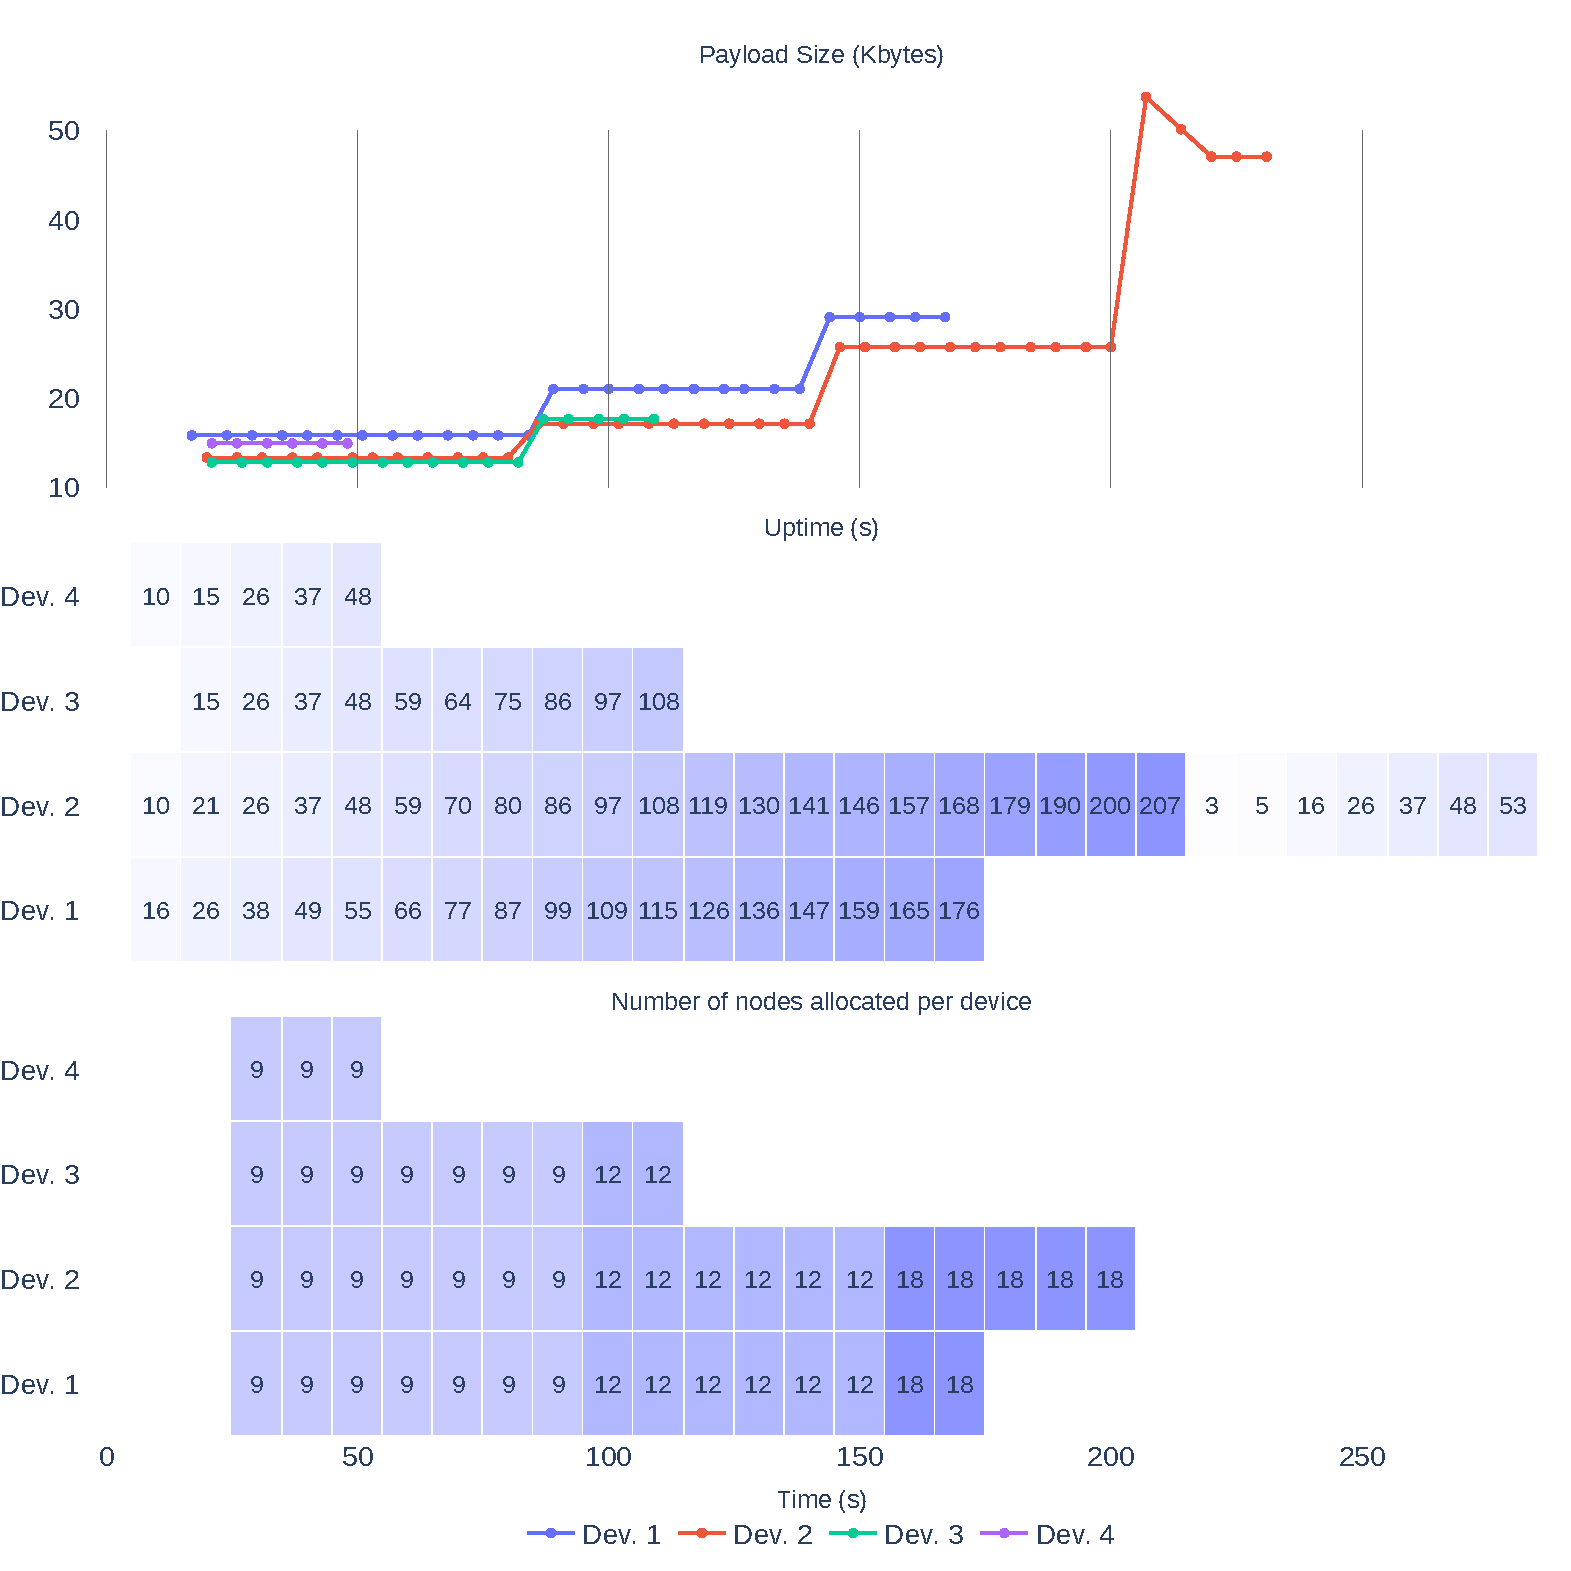
\includegraphics[width=\linewidth]{experiences/A-reorchestration_phys/reorchestration_phys.pdf}
    \caption{ES1-B measurements}
    \label{fig:experiment_a_phys_graph}
\end{figure}

The payloads and number of \textit{nodes} assigned through the experiment are very similar to the experiment \textbf{ES1-A} \seefigureref{fig:experiment_a_phys_graph}. However, it is noticeable that \textit{Device 2} (the last remaining active device), fails when receiving the final-step payload --- which contains the code for all the \textit{nodes} of the system, since no other device is available. 

The device constrained memory cannot handle the payload size, so it \textsc{fail-safe}s, informing the system that there was an \textit{Out-of-Memory} error, which results in \textit{Orchestrator node} assigning fewer \textit{nodes} to the device. However, the is no more available devices to assign the remaining nodes, resulting in an non-functional orchestration.

%%%%%%%%%%%%%%%%%%%%%% Exp C %%%%%%%%%%%%%%%%%%%%%%

\subsubsection{ES1-C}

\begin{figure}[h]
    \centering
    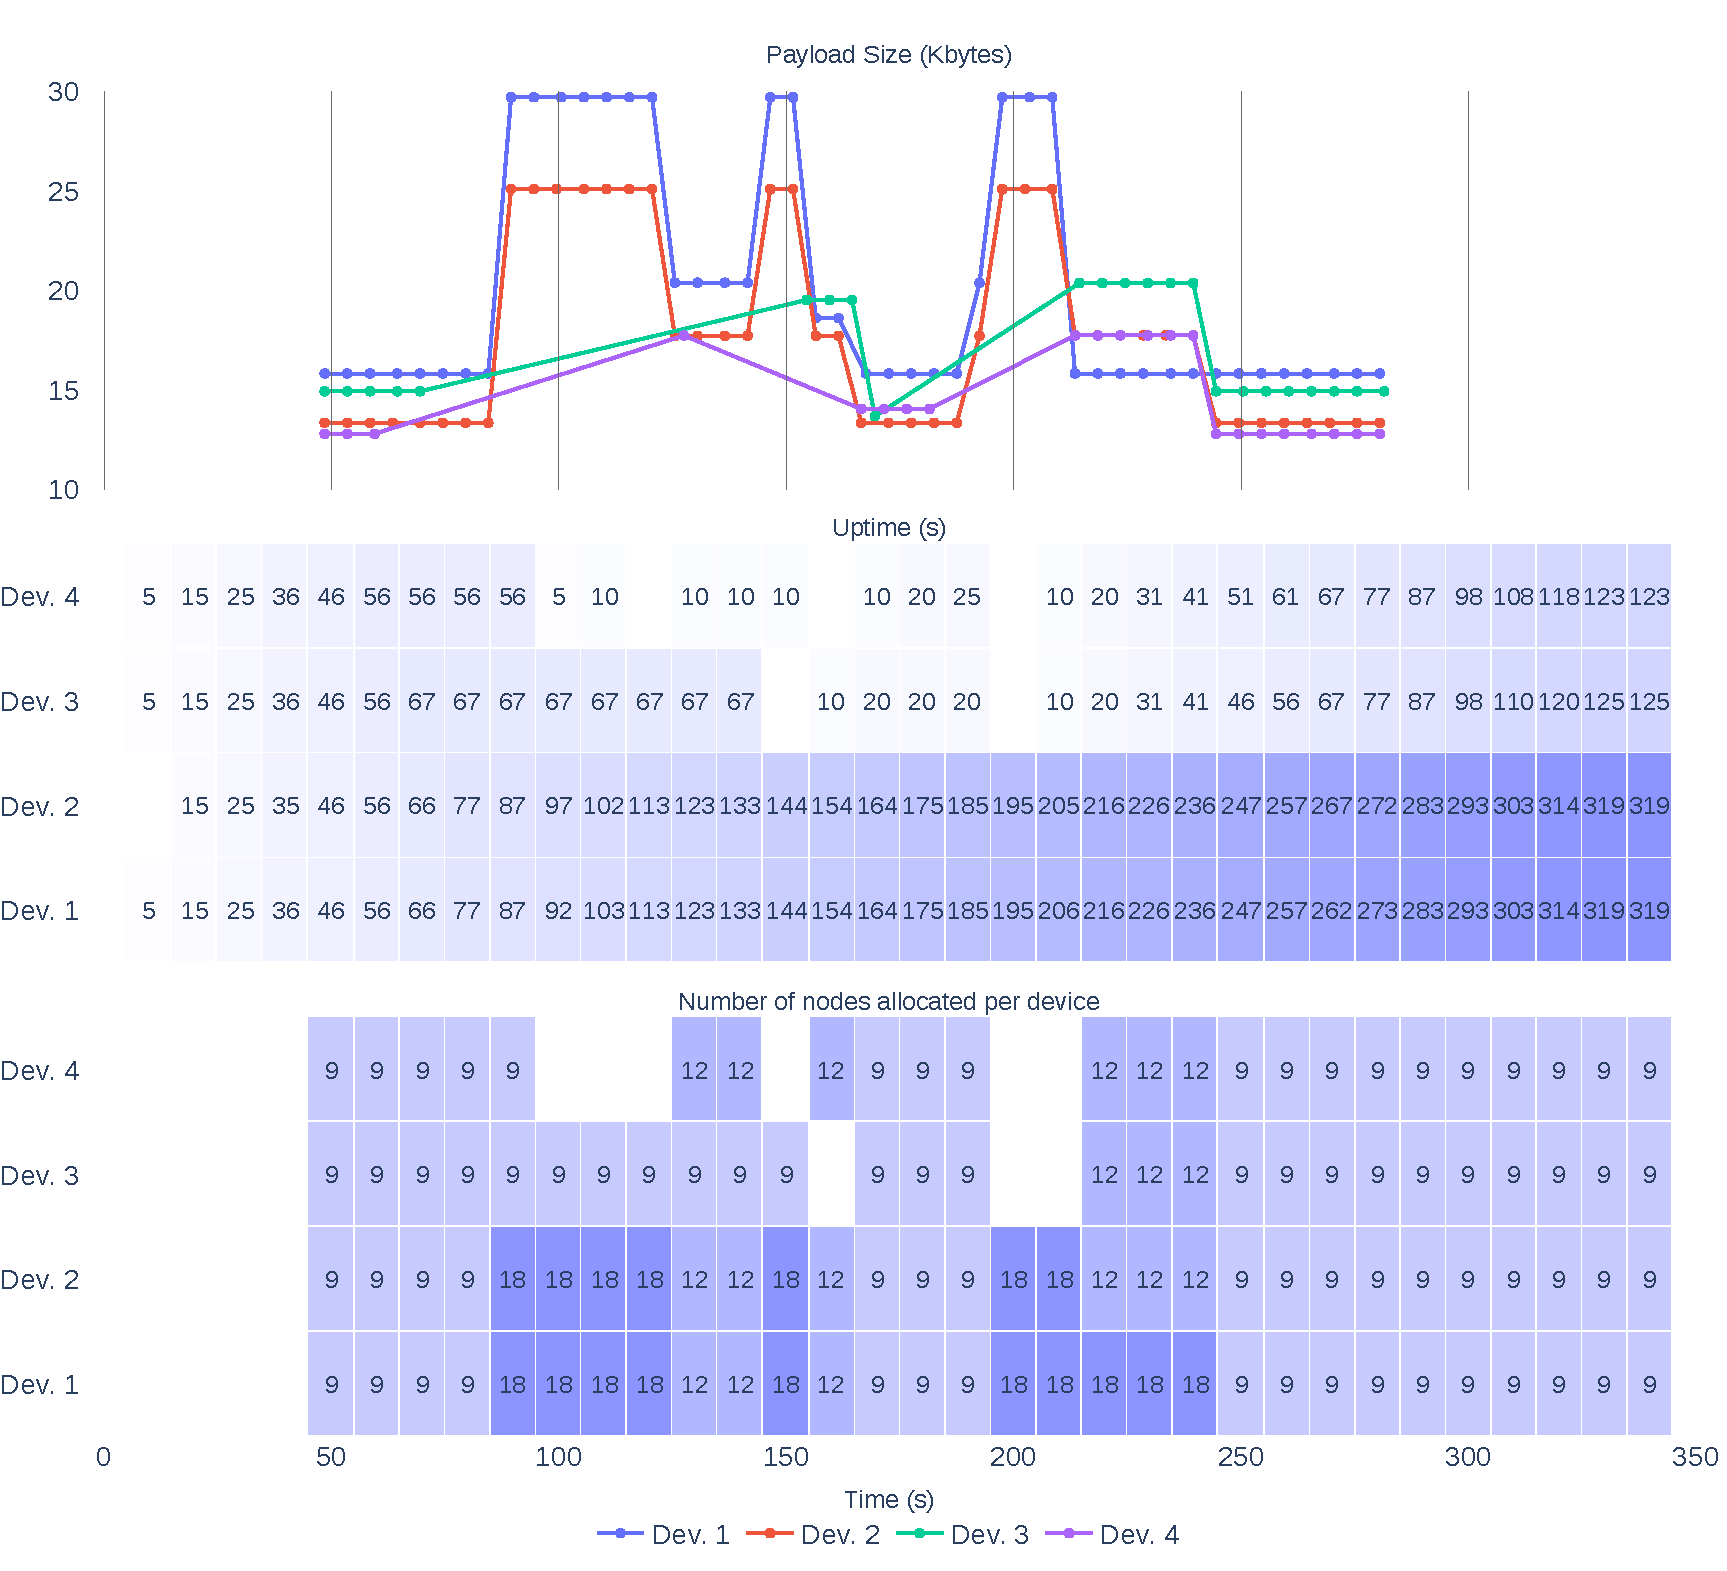
\includegraphics[width=\linewidth]{experiences/B-reorchestration-inconsistent/reorchestration_inc.pdf}
    \caption[ES1-C measurements]{ES1-C measurements.}
    \label{fig:experiment_b_graph}
\end{figure}

Similar to \textbf{ES1-A} and \textbf{ES1-B}, this experiment focuses on testing the system's ability to adapt when devices fail and then recover. In \figureref{fig:experiment_b_graph}, \textit{Device 3} and \textit{Device 4} fail early, and the system recovers, allocating the \textit{nodes} assigned to them to other devices. \textit{Device 4} recovers around the 100s, fails again and then recovers. The system did not catch this change since it was swift, and the system only re-orchestrates the second time \textit{Device 4} recovers. During this experiment, \textit{Device 3} and \textit{Device 4} continue to fail and recover, and the system always re-configures itself.

This re-orchestration ability when a device recovers can be taxing to the functionality of the system. If a device is continuously failing and recovering, the system will always try to adapt itself, halting its functionality to orchestrate.

%%%%%%%%%%%%%%%%%%%%%% Exp D %%%%%%%%%%%%%%%%%%%%%%

\subsubsection{ES1-D}

The memory constraints of IoT devices can negatively impact the functioning of the system, by raising memory errors when writing the received script into the device SPI flash. This experiment verifies how the system recovers and adapt to the device's memory constraints.

\begin{figure}[h]
\centering
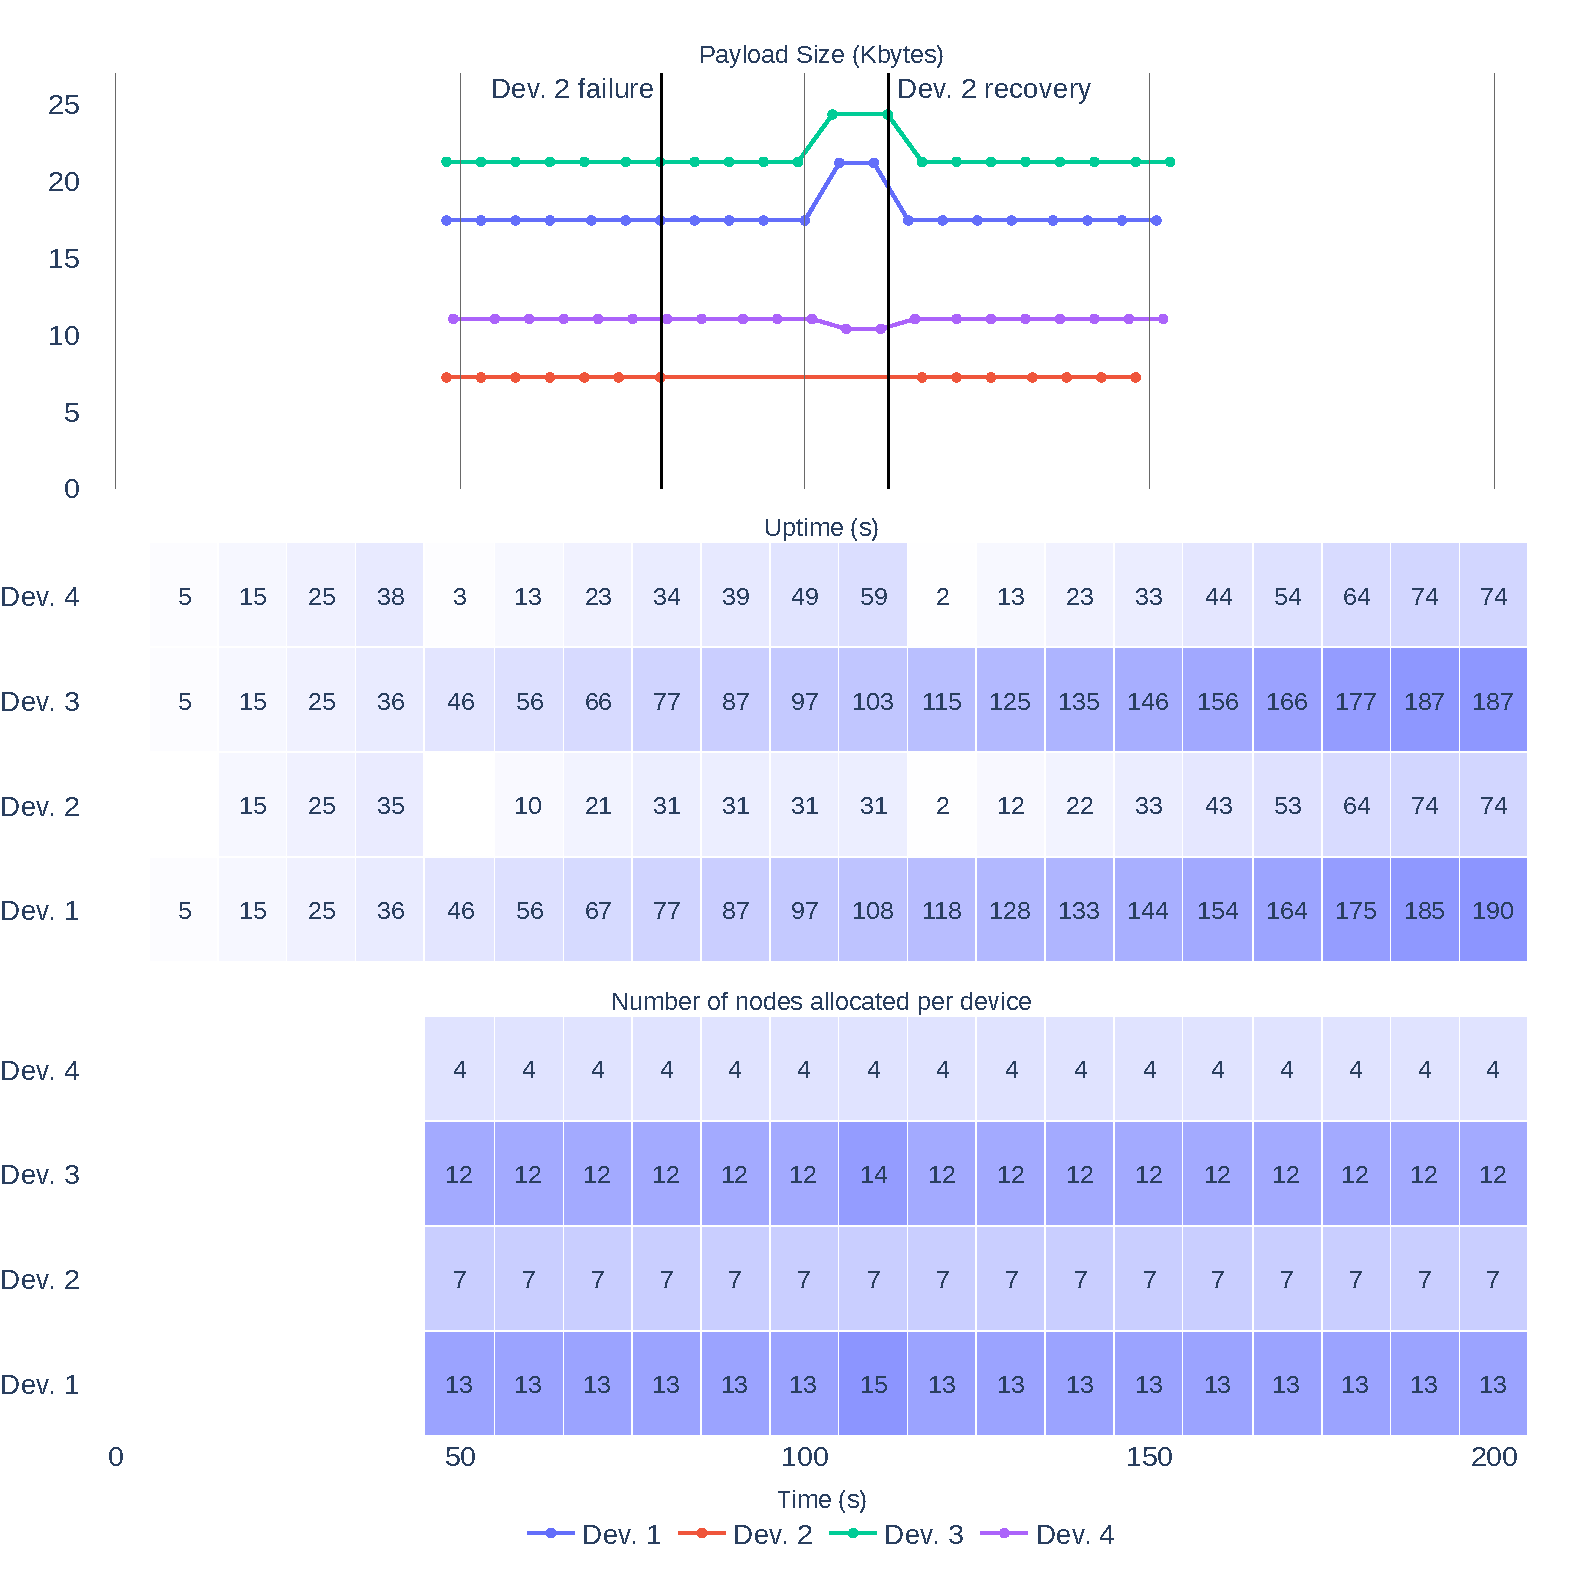
\includegraphics[width=\linewidth]{experiences/C-memory_error_on_write/memory_write.pdf}
\caption[ES1-D measurements]{ES1-D measurements.}\label{fig:experiment_c_graph}
\end{figure}

\figureref{fig:experiment_c_graph} shows the constrained memory of the \textit{Device 2} and \textit{Device 4}. When the first assignment is made, at approx. 50 seconds, both these devices \textsc{fail-safe} due to \textit{Out-of-Memory} errors. The number of \textit{nodes} present on these devices are the ones assigned after they communicate to the orchestrator their limitations. 

To assess if the system saves information about the limitations of the devices, one of them was turned off and later turned on \seefigureref{fig:experiment_c_graph}. As it can be observed, \textit{Device 2} uptime stops increasing around the time of the event and its \textit{nodes} are distributed by the other devices, except for \textit{Device 4}, which is memory constrained. After the recovery of \textit{Device 2}, the system re-orchestrates and the same number of \textit{nodes} is assigned to the devices. However, \textit{Device 4} failed when \textit{Device 2} recovered, which implies that the system repeated the process assignment process, ignoring the previously known information about memory constraints. This is a limitation of the system since it would be beneficial to save memory constraints of devices when they fail and recover, preventing the repetition of the orchestration iteration.

%%%%%%%%%%%%%%%%%%%%%% Exp E %%%%%%%%%%%%%%%%%%%%%%

\subsubsection{ES1-E}

In addition to the handling of memory limitations, it is expected that the system can handle a damaged device which has a memory leak issue. \textit{Device 2} was modified to always generate an \textit{Out-of-Memory} error after a random period. The system should be able to exclude this device during the assignment process.

\begin{figure}[h]
\centering
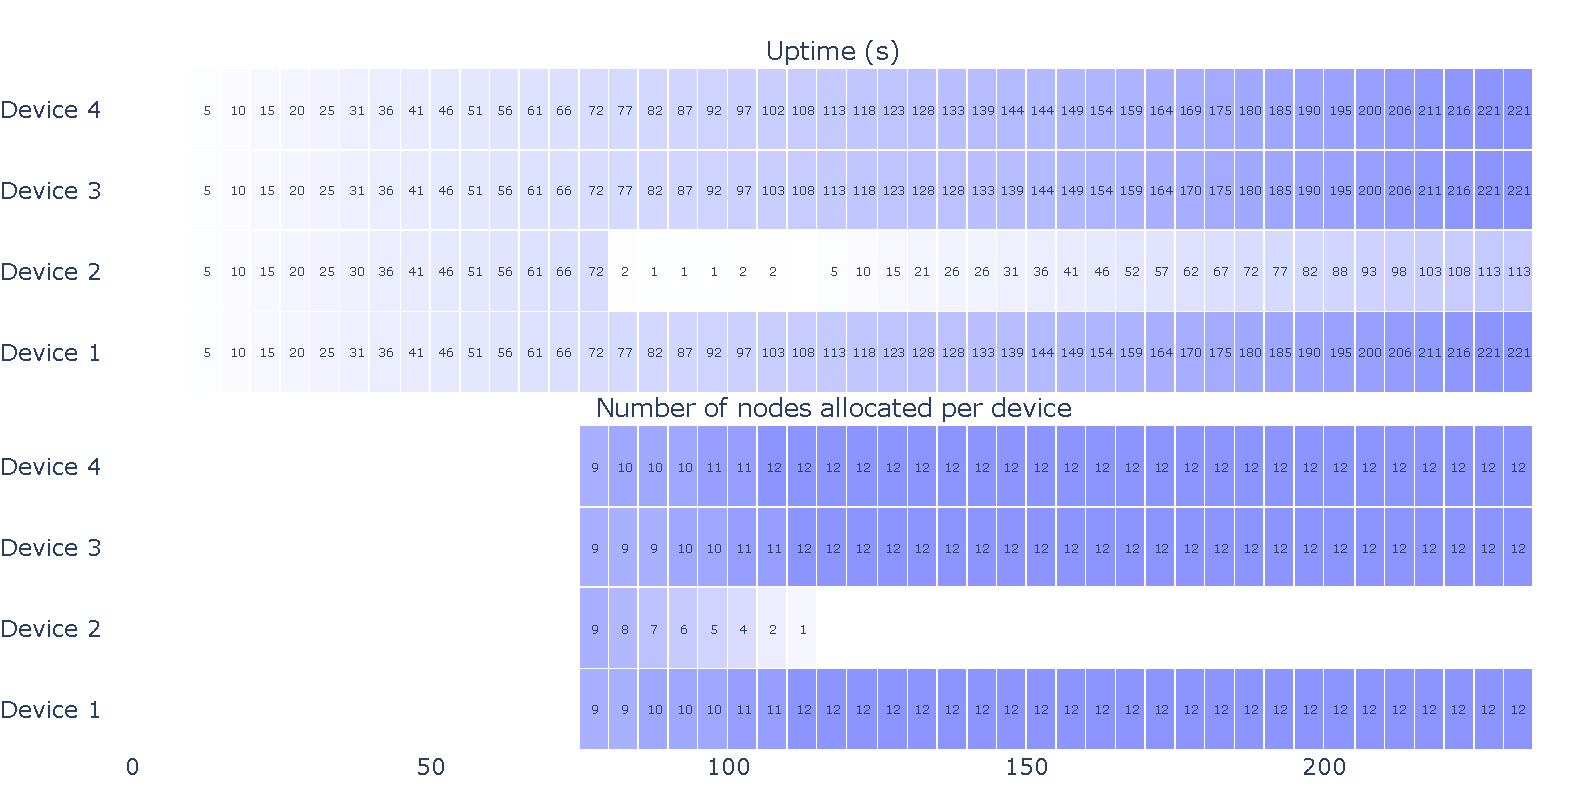
\includegraphics[width=\linewidth]{experiences/D-memory_error_random/memory_random.pdf}
\caption[ES1-E measurements]{ES1-E measurements.}\label{fig:experiment_d_graph}
\end{figure}

\figureref{fig:experiment_d_graph} shows that \textit{Device 2} is consistently failing after the first assignment of \textit{nodes}, at approx. 75 seconds. The number of \textit{nodes} assigned decreases, until no \textit{node} is assigned and the device is excluded from consideration. This is an iterative process, in which the system will decrease the number of \textit{nodes} it assigns to a device if the device communicates an \textit{Out-of-Memory} to the orchestrator. Eventually, the minimum number of \textit{nodes} the device can handle is zero, excluding the device from the assignment process.

%%%%%%%%%%%%%%%%%%%%%% Exp F %%%%%%%%%%%%%%%%%%%%%%

\subsubsection{ES1-F}

To further assess the resilience of the system to \textit{Out-of-Memory} errors, a \textit{node} was deliberately injected that causes such error in specific devices. It is expected that the system re-orchestrate and converge to a solution where the specific \textit{nodes} are assigned to devices not affected by them. In turn, the devices affected by these \textit{nodes} should have fewer \textit{nodes} assigned. The system and devices do not know that a specific \textit{node} is creating the \textit{Out-of-Memory} errors and interpret the error as a device problem.

\begin{figure}[H]
\centering
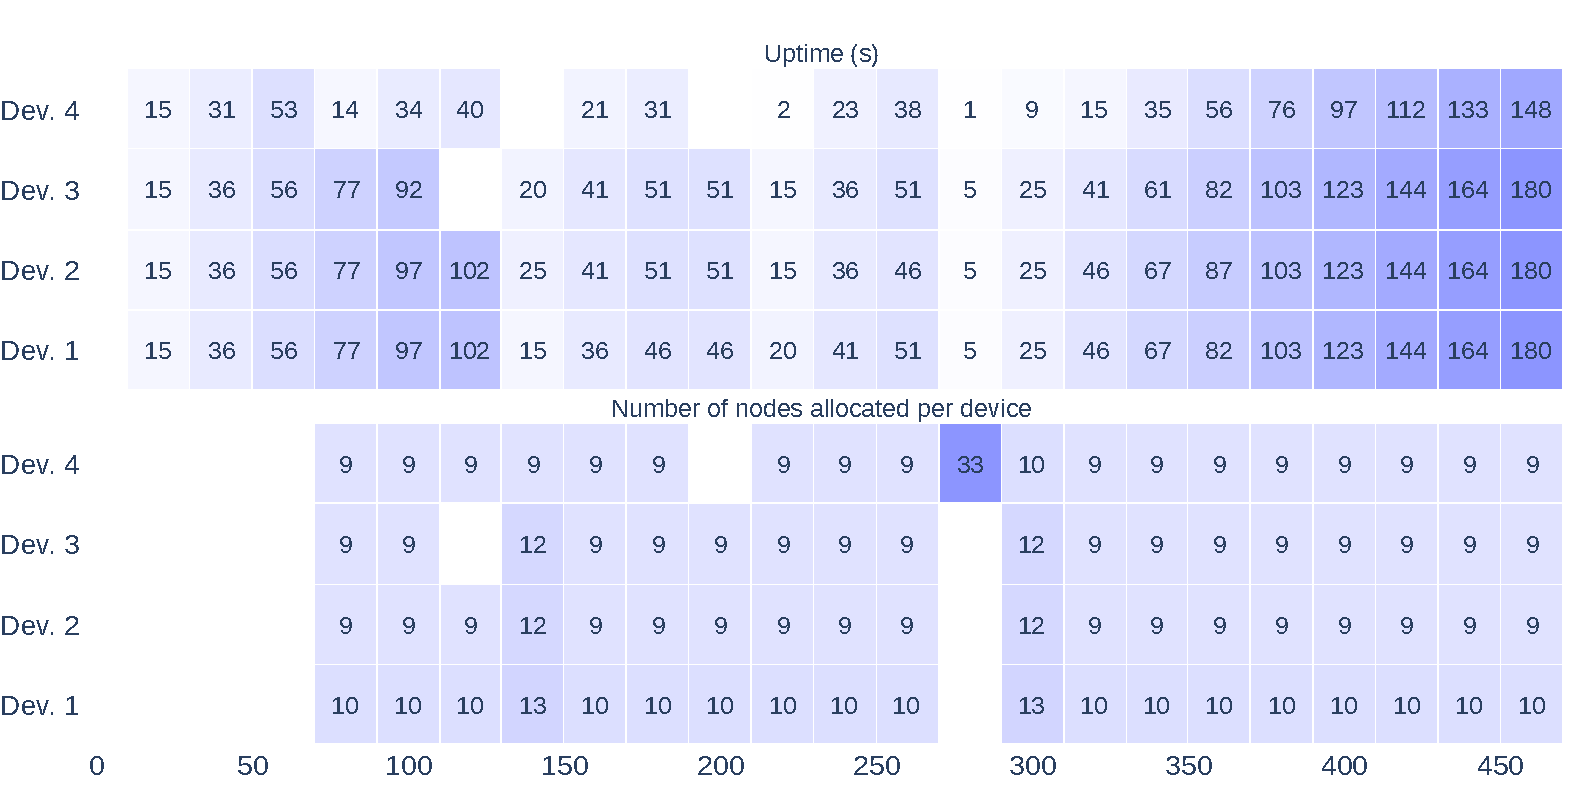
\includegraphics[width=\linewidth]{experiences/E-memory_error_node_failure/memory_failure.pdf}
\caption[ES1-F measurements]{ES1-F measurements.}\label{fig:experiment_e_graph}
\end{figure}

Since the first orchestration could be correct by sheer chance, meaning that these faulty \textit{nodes} would be assigned to devices not affected by them, we forced the system to re-orchestrate. The devices were all turned off and on in different order, repeating three times. \figureref{fig:experiment_e_graph} shows these on/off events at approx. 125, 200 and 275 second timestamps. It is important to note that the devices affected by the faulty \textit{nodes} are \textit{Device 2} and \textit{Device 4}.

The event we aim to test occurs at approx. 300 seconds. As it can be seen \seefigureref{fig:experiment_e_graph}, \textit{Device 4} is assigned 10 \textit{nodes}. The uptime of \textit{Device 4} resets in this small time period --- the next uptime is less than 20 seconds --- meaning that an \textit{Out-of-Memory} occurred and the device performed a \textsc{fail-safe}. The system updates, allocating the 10 \textit{nodes} previously assigned to \textit{Device 4} through all the available devices. Since \figureref{fig:experiment_e_graph} shows the data in intervals of 20 seconds, the assignment in \textit{Device 4} happens before the assignment present in the other devices.

When the system receives information that \textit{Device 4} is available again, it already knows that it has a limitation, so it only assigns 9 \textit{nodes} to it. It can be seen that missing \textit{node} is assigned to \textit{Device 1}. Since \textit{Device 4} does not \textsc{fail-safe}, the \textit{node} assigned to \textit{Device 1} must have been the faulty one.

%%%%%%%%%%%%%%%%%%%%%% Exp G %%%%%%%%%%%%%%%%%%%%%%

\subsubsection{ES1-G}\label{sec:experiment_f}

To assess our system's limits, we proceed to inject constant failures in the available devices. Every second, each device has a 5\% probability of becoming unavailable from 0 to 10 seconds. During this period, the device is unresponsive to the orchestrator requests and, when recovered, announces itself.

\begin{figure*}[h]
    \centering
    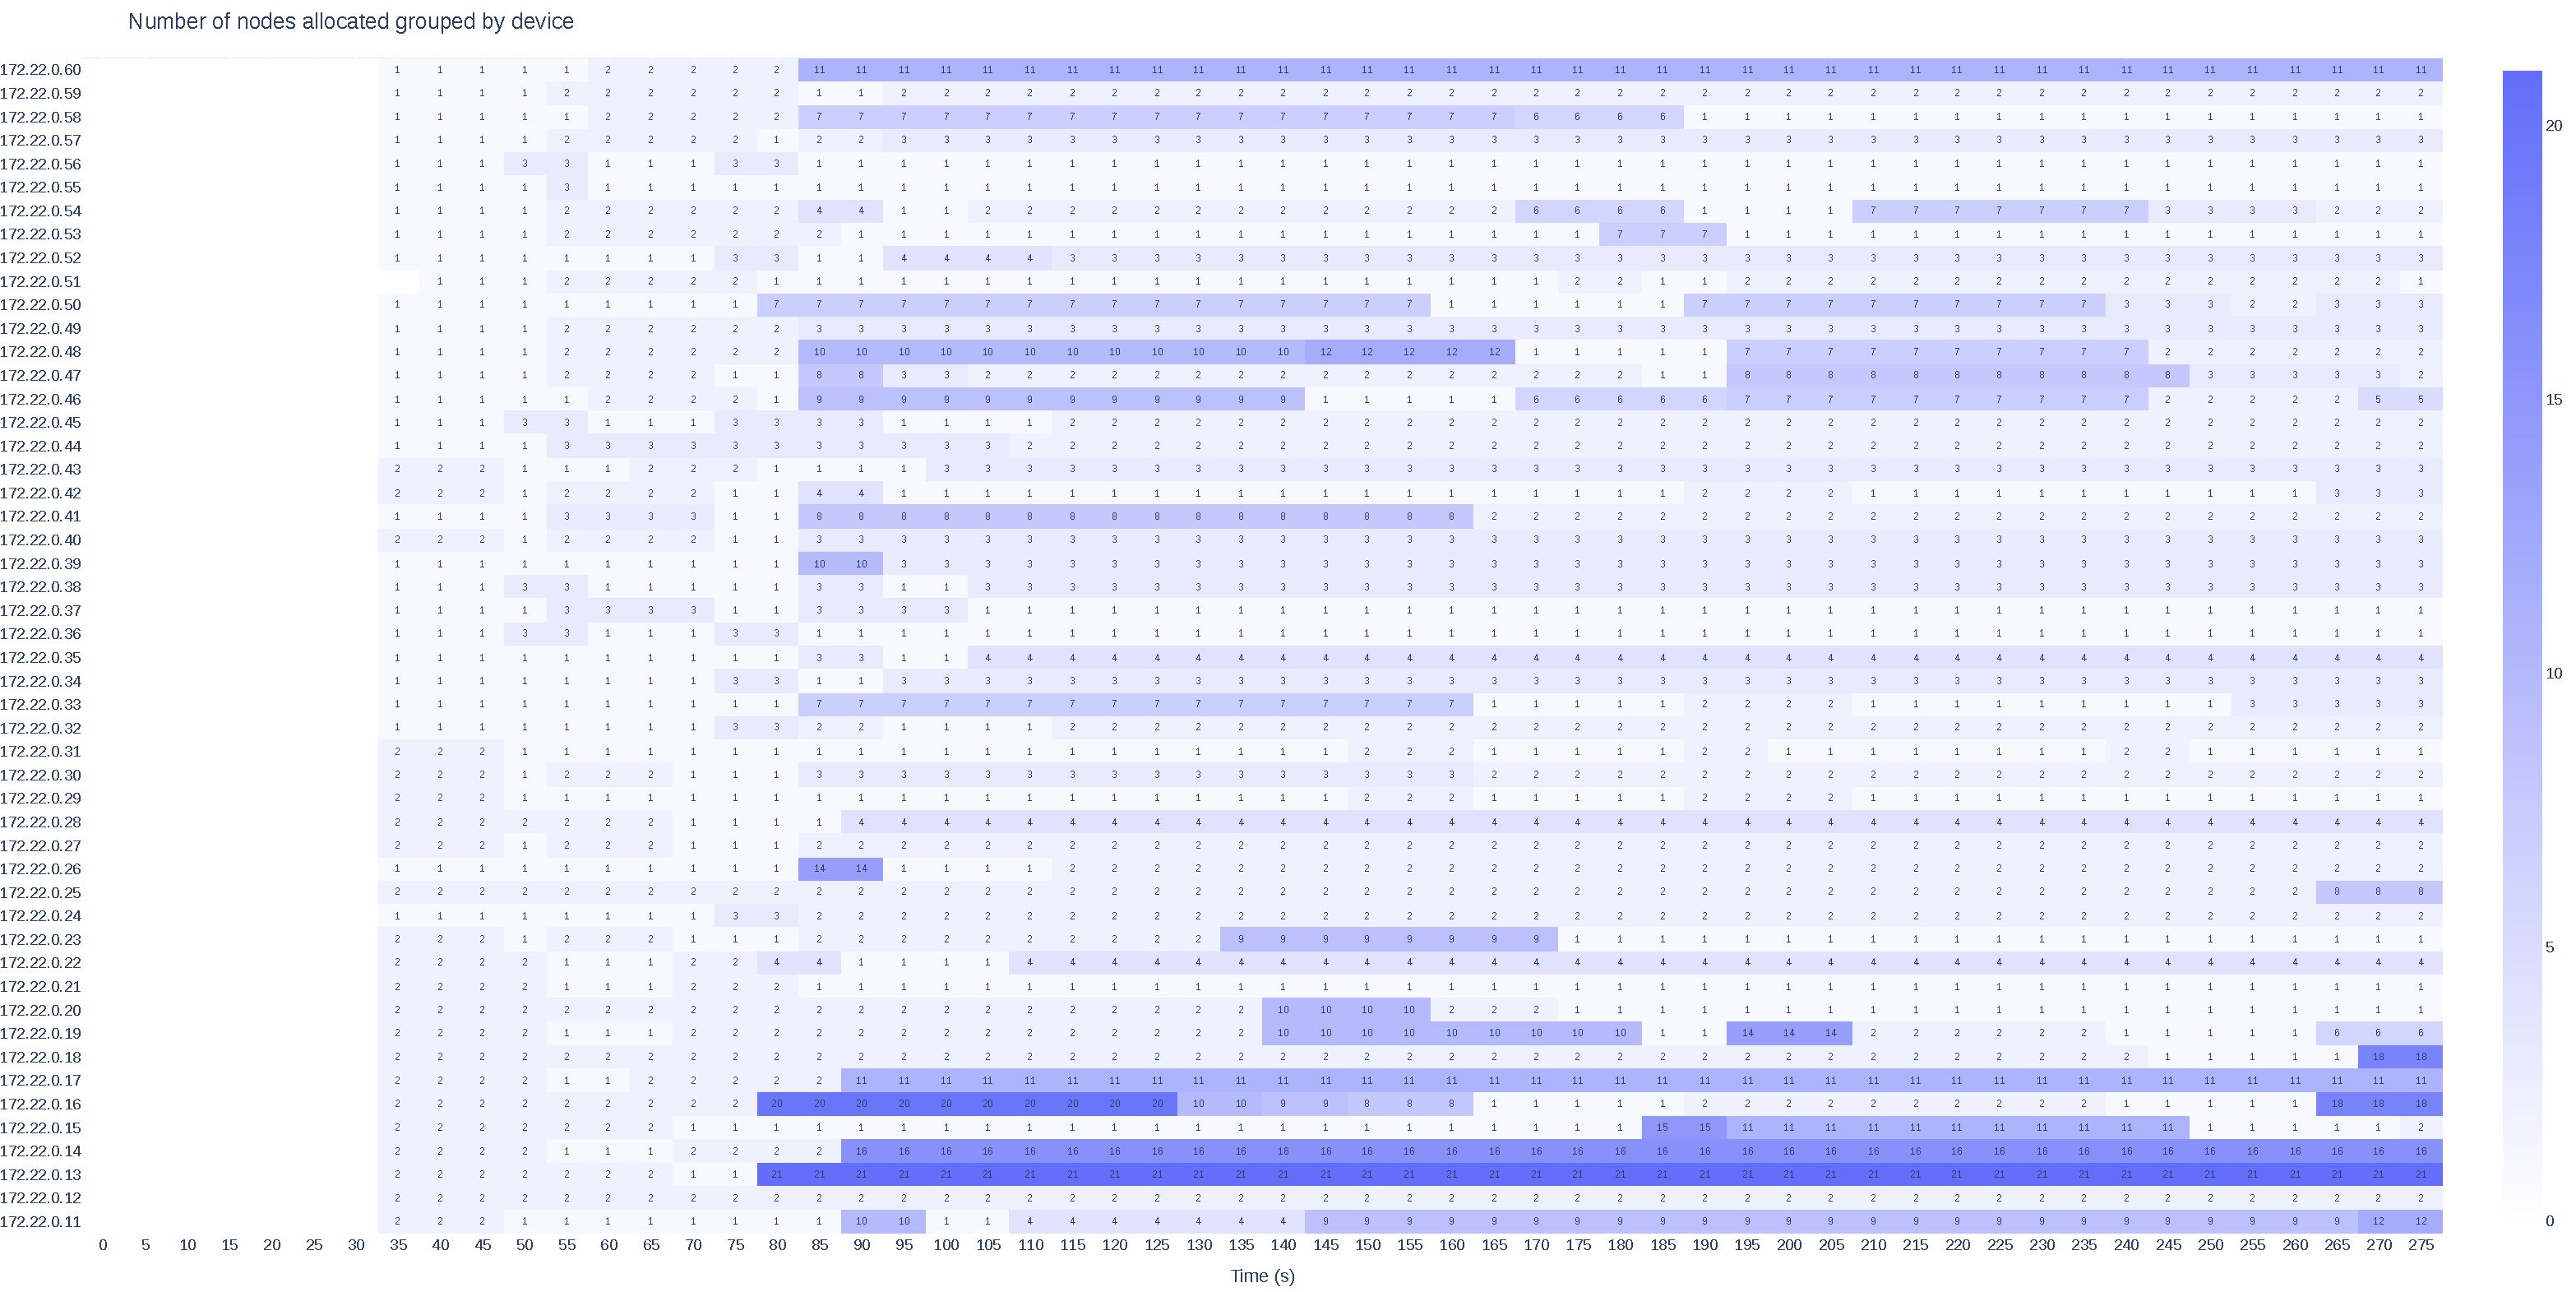
\includegraphics[width=\textwidth]{experiences/F-stress_test/nodes_heatmap.pdf}
    \caption[Nodes assignment distribution]{Nodes assignment distribution}\label{fig:stress_test_nodes}
\end{figure*}

\figureref{fig:stress_test_nodes} shows that the system is kept continuously re-orchestrating, and once the majority of devices failed, the system becomes unstable. It is important to note that, similar to previous experiments, once a device fails, the number of \textit{nodes} does not update to zero. We then conclude that devices with the same number of \textit{nodes} throughout the duration of the experiment failed early on and kept failing, not accepting another assignment by the orchestrator.

\begin{figure}[H]
\centering
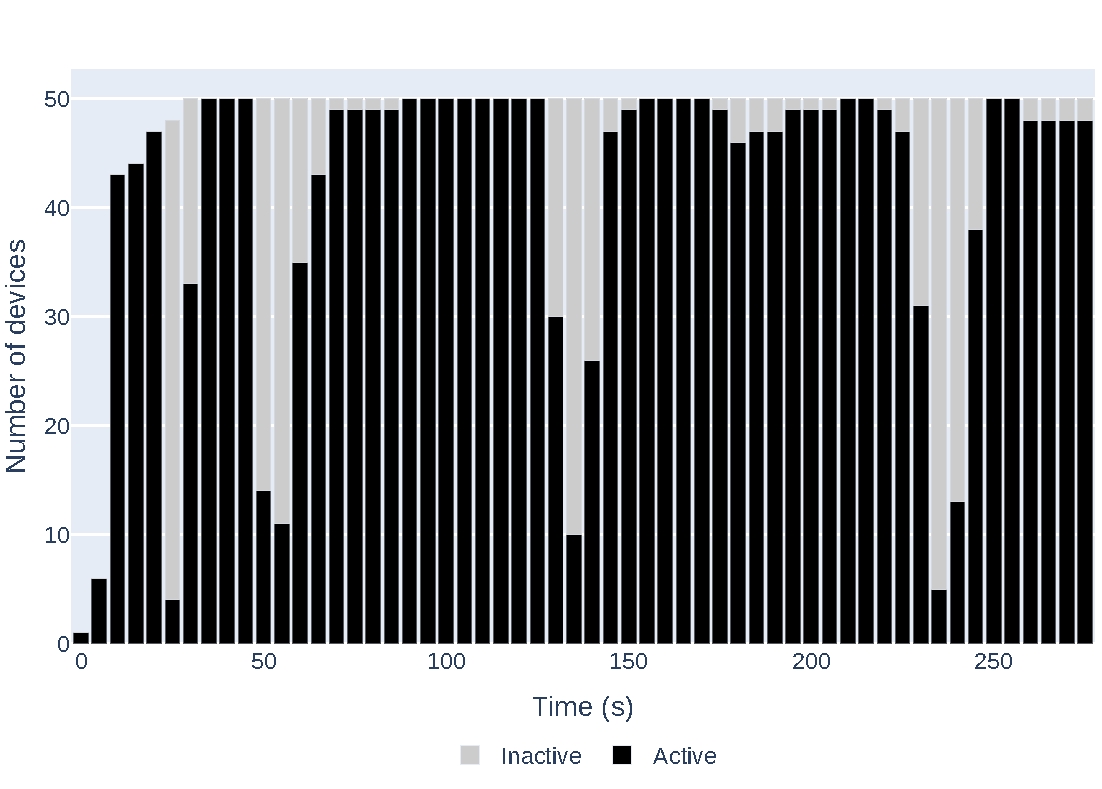
\includegraphics[width=\linewidth]{experiences/F-stress_test/status.pdf}
\caption[Number of devices active and inactive]{Number of devices active and inactive}\label{fig:stress_test_status}
\end{figure}

At approx. 100 seconds, it can be noted in \figureref{fig:stress_test_status} a period where all devices were available. However, the \textit{node} assignment in \figureref{fig:stress_test_nodes} does not converge during that time period. The reason for this behaviour is that the system will re-orchestrate when a device becomes available. Since each device announces itself individually, each announcement triggers a new orchestration. This process takes time and results in several failed orchestrations due to outdated data on the device's operating status. 

The outdated data issue has been identified as a current limitation of the system, making it vulnerable to a possible Denial-of-Service (DoS) attacks in the form of an excess of status activity from the devices. This constant orchestration is also taxing for the devices, causing an overload of received assignments that will never make the system function as a whole.

%%%%%%%%%%%%%%%%%%%%%%%%%%%%%%%%%%%%%%%%%%%%

\subsection{ES2: Experimental Tasks}\label{sec:discussion_scenario2}

To benchmark our approach we proceed to experiment with a \textit{flow} that consists on passing a message through several devices, recording the elapsed time for the message to pass through all the devices.

\begin{figure}[h]
\centering
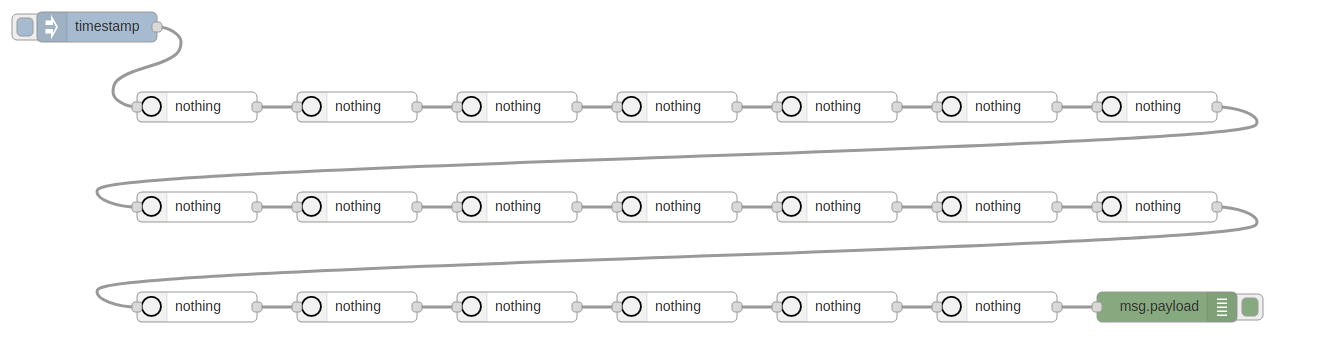
\includegraphics[width=\linewidth]{scenario2.png}
\caption[Node-RED implementation of scenario 2]{Node-RED implementation of scenario 2}\label{fig:scenario2_node_red}
\end{figure}

The ES2 implementation in Node-RED can be seen in \figureref{fig:scenario2_node_red}. The \texttt{NOP} (in the image with the name \textit{nothing}) \textit{nodes} execution consists of only redirecting their input to their output. A message containing only the current timestamp is inserted into the system by triggering the \textit{Inject} \textit{node}, and the same message is expected to appear in the Node-RED \textit{Debug} console (using the \textit{Debug} node).

\captionsetup{belowskip=12pt,aboveskip=4pt}
\begin{table}[ht]
    \centering
    \resizebox{\textwidth}{!}{%
    \begin{tabular}{ l  r  r  r  r  r  r }
        \toprule
        \textbf{Label} & \textbf{Min}  & \textbf{Q1} & \textbf{Q2}  & \textbf{Avg} & \textbf{Q3} & \textbf{Max}\\
        \midrule
        \textbf{ES2-A}: Node-RED original & 3 & 8 & 10 & 10 & 13 & 15 \\
        \textbf{ES2-B}: Node-RED + MQTT & 134 & 353 & 431 & 489 & 711 & 883 \\
        \textbf{ES2-C}: Node-RED modified + Dockers (same host) & 1217 & 1260 & 1318 & 1400 & 1574 & 1665 \\
        \textbf{ES2-D}: Node-RED modified + Dockers (different host) & 1445 & 2332 & 2536 & 2392 & 2708 & 3059 \\
        \textbf{ES2-E}: Physical + MQTT & 3616 & 4031 & 4142 & 4133 & 4372 & 4452 \\
        \textbf{ES2-F}: Node-RED modified + MQTT + Physical + Firmware & 4168 & 4357 & 4569 & 4751 & 5088 & 5940 \\
        \bottomrule
    \end{tabular}
    }
    \caption{Scenario 2 results}
    \label{tab:scenario2_table}
\end{table}{}

This experiment was run with different configurations (\textbf{ES2-A} to \textbf{ES2-F}) to assert the impact of each modification/module, as described in \sectionref{sec:experiments}. Each experiment was replicated ten times, and the resulting measurements are shown in \tableref{tab:scenario2_table}.

\begin{figure}[h]
\centering
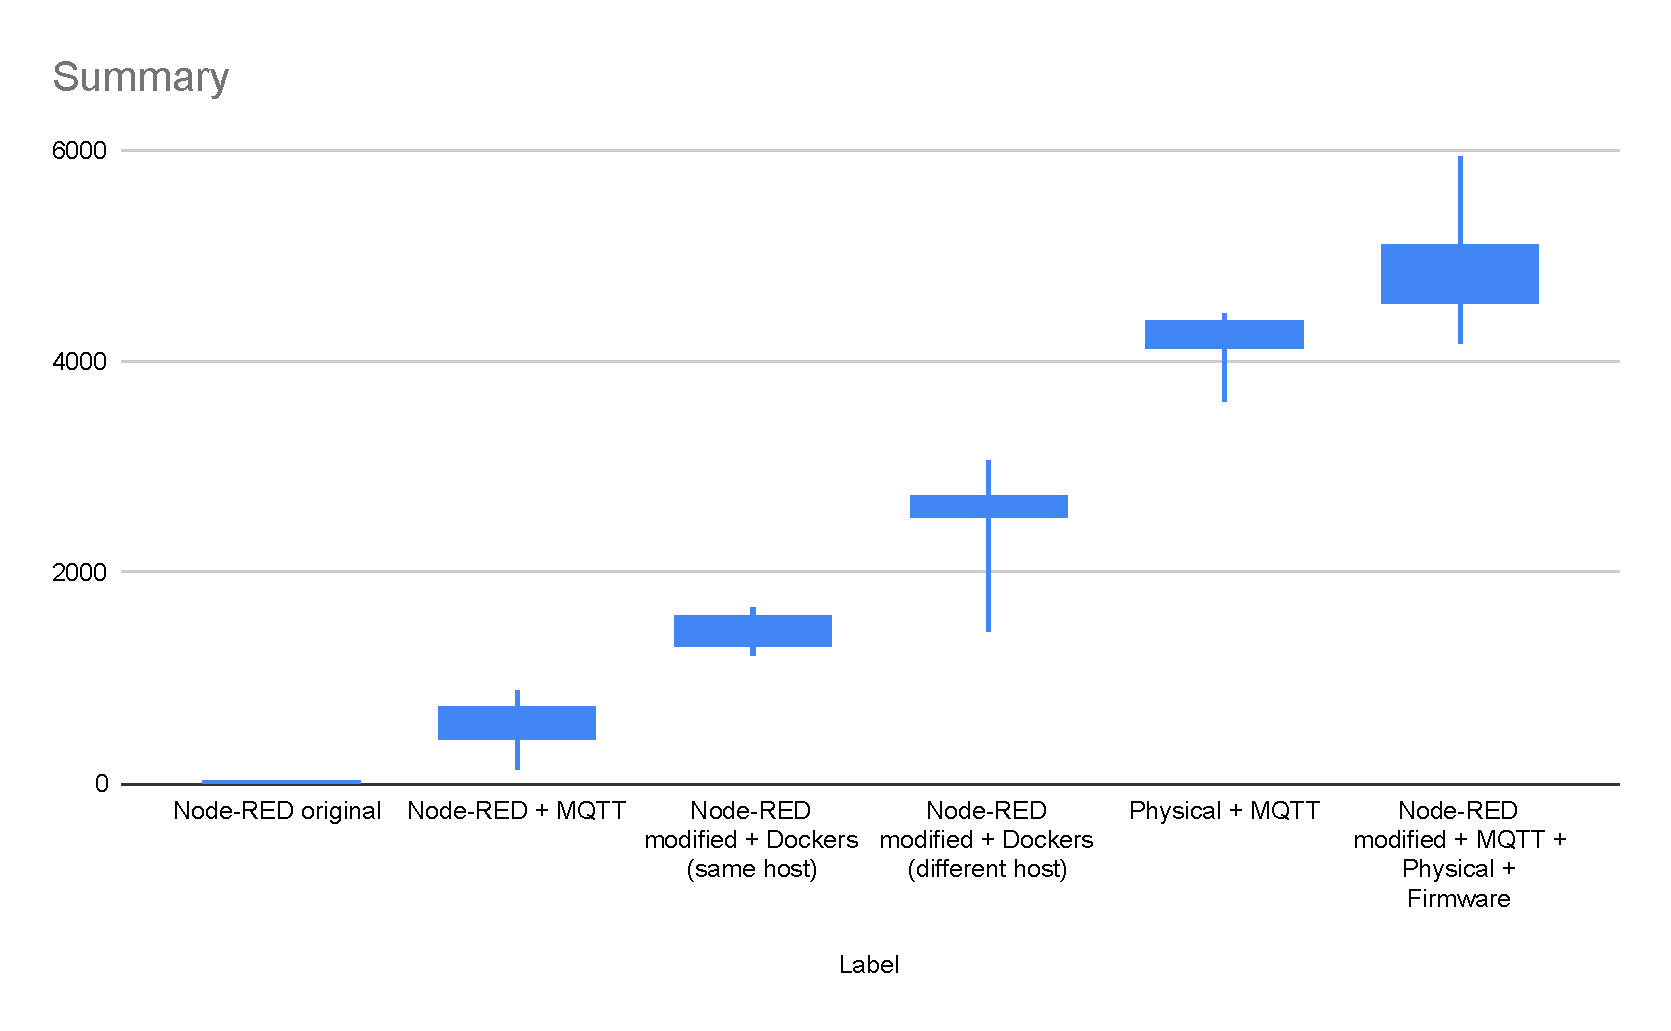
\includegraphics[width=\textwidth]{scenario2_graph.pdf}
\caption[ES2 results.]{ES2 results.}\label{fig:scenario2_candlestick}
\end{figure}

\figureref{fig:scenario2_candlestick} demonstrates that the developed solution introduces overhead in communicating between nodes. However, given the other experiments, it is possible to conclude that this lack of efficiency is caused not by the created firmware, but because of the stack of communication the message travels through, as well as the nature of MicroPython. 

When the decentralization is applied inside Node-RED (\cf \textbf{ES2-B}), without running any MicroPython, it is possible to see that the introduction of the MQTT communication (Mosquitto broker) running in the same host causes some latency. The introduction of Dockers running the firmware in the same host as the Node-RED instance and MQTT causes additional latency (\cf \textbf{ES2-C}), making it possible to conclude that the MicroPython-based developed firmware also delays the communication. By repeating the same experiment but with the broker running in another machine (same network) (\cf \textbf{ES2-D}), it is noticeable that the times are more spread out and the overall latency of the system increases. As the Node-RED and the broker run in different machines connected over Wi-Fi, we conclude that this is the leading cause for the additional delay in communications. 

The experiment was repeated in physical devices: (1) by running a simple code in the MicroPython flashed devices and injection of messages directly in the broker (\cf \textbf{ES2-E}), and (2) by using our approach as a whole, with the modified Node-RED and firmware in the devices (\cf \textbf{ES2-F}). The communication and MicroPython overhead in the last experiment made (\cf \textbf{ES2-F}, our approach), is 4000 milliseconds, which will be attributed to variable \textit{x}. The overhead of using the created MicroPython firmware, variable \textit{y}, is the total time minus the \textit{x} variable, which is ~750 milliseconds. The results allow us to conclude that the use of physical devices produce higher times (as expected), but that the developed firmware has little impact in them.

We can conclude that our \textit{proof-of-concept} is slower than the original Node-RED, but the latency introduced are due to communication overheads and latency of the MicroPython firmware. Some overhead was introduced by the developed firmware, but it is not significant. Although the communication changes are necessary for the decentralization of the system, the MicroPython firmware latency could be reduced with the use of another firmware, for example C-based.

\section{Hypothesis Evaluation}\label{sec:evaluation_hypothesis}

This evaluation process aimed to prove the hypothesis presented in Section \ref{sec:main_hypothesis}. Given the results of the experiments with our proof-of-concept, we conclude that the challenges that we focused on were tackled, more specifically the decentralization of computation, with the handling of the device's memory constraints and failures, and dynamic adaptation of the system (self-reconfiguration). The attributes mentioned in \sectionref{sec:main_hypothesis} were evaluated, resulting in the following conclusions:

\begin{itemize}
    \item \textbf{Resilience}: The developed solution is moderately robust, handling device failures and memory constraints dynamically at runtime. However, there are some limitations to this robustness. As demonstrated in Section \ref{sec:experiment_f}, the system reaches a maximum point of adaptability when several devices fail and recover continually. Possible solutions to this problem are mentioned in \sectionref{sec:future_work}.
    \item \textbf{Efficiency}: Although the developed solution is slower than the original Node-RED system. However, the increased latency is due to the change in the communication channel, which introduces some extra latency (as expected). Despite this, the developed modules, such as the orchestrator and the device's firmware introduce little latency to the latency of the whole system.
    \item \textbf{Elasticity}: The solution handles a different number of devices, as it was demonstrated in the experiments. It also handles the number of devices changes throughout the lifespan of the system, adapting the orchestration to the number of devices available.
\end{itemize}

In summary, the developed solution is more scalable than a centralized one, dealing with a dynamic number of devices while taking advantage of their computational capabilities. It is also robust enough to handle the failures and constraints of these devices. The developed solution introduces some overheads, but its major factor of latency is due to factors external to the developed firmware, which are required to achieve a decentralized solution.

\section{Lessons Learned}\label{sec:evaluation_lessons_learned}

There were several changes made to the developed solution during the evaluation process. These changes were necessary to allow the capture of data that was later used to generate charts and reach conclusions. The lessons learned during this process consisted in figuring out how to build a framework that supported sending and capture of data, its aggregation and visualization and which metrics to capture, which ended up being the majority of the ones we identified.

Each device was modified to allow them to send metrics to MQTT topics, which in turn were captured by a bridge that populated an InfluxDB database. This database supplied a Grafana dashboard, where the data from the evaluation was exported from. In addition to this, both the devices and Node-RED sent data to a Logstash, which supplied a Kibana instance using Elastic Search. These logs were sometimes useful to understand the events happening in the devices and orchestrator in more complex experiments.

The setup necessary for this process required modifying the developed solution. It was an iterative process in which the number of metrics captured increased each time an experiment was made.

\section{Conclusions}\label{sec:evaluation_conclusions}

This Chapter presents the results from the evaluation process of the developed solution. \sectionref{sec:scenarios} starts by defining the scenarios and \sectionref{sec:experiments} details the experiments that were used to test the tool and its features. \sectionref{sec:evaluation_discussion} analyzes the results from the experiments and reaches several conclusions about the developed solutions: (a) it detects device failures and memory constraints and automatically adapts itself in order to keep functioning, (b) it is slower than the original Node-RED but the overheads introduced are caused by communication and MicroPython latency, and (c) it adapts itself to different number of devices, which may vary during the lifespan of the system.

However, during \sectionref{sec:evaluation_discussion} several limitations to the solution were found, such as (a) its inability to handle the constant failure and recovery of devices, creating a constant state of adaptation that does not allow the system to converge on an orchestration and (b) the lack of persistence in device's memory constraints information when they fail, causing orchestration iterations to be repeated when the device becomes available again.

Given the previous analysis, \sectionref{sec:evaluation_hypothesis} reflects on the presence of the attributes defined in \sectionref{sec:main_hypothesis} in the developed solution. Finally, \sectionref{sec:evaluation_lessons_learned} reflects on the lessons learned during the evaluation process.

